\section{Concept of Root Locus}

\begin{frame}
\frametitle{Concept of the method}
In this chapter the Root Locus Method is presented. This technique shows how changes in the system's feedback characteristics and other parameters influence the pole locations. The method permits us to plot the locus of the closed-loop pole locations in the s-plane as a parameter varies, which will produce a root locus (hence the name of the technique).\\
\vspace{1em}
It is very important to understand the background of root loci: how they take their shape, why they are useful, ... Therefore, we start this chapter by explaining the concept of the Root Locus Technique. Next we explain how to sketch a root locus. Finally we will give some examples in MATLAB.
\end{frame}

\begin{frame}
\frametitle{Concept of the technique}
	We begin with the basic feedback system, shown in the figure below:
	\begin{figure}
		\centering
		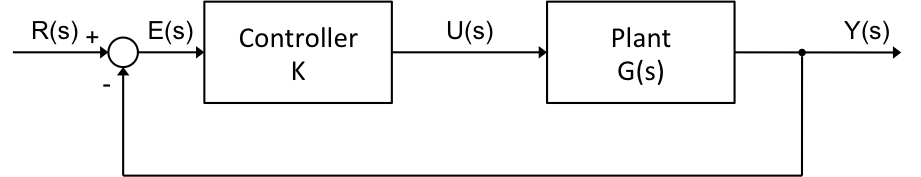
\includegraphics[width=1\linewidth]{closed_loop_diagram}
	\end{figure}
	The closed-loop transfer function is:
	\begin{center}
		$H(s) = \frac{Y(s)}{R(s)} = \frac{KG(s)}{1 + KG(s)}$.
	\end{center}
\end{frame}

\begin{frame}
\frametitle{Concept of the technique}
	Looking at this transfer function, we can conclude that the closed-loop roots depend on the gain $K$. We can now plot the locus of all possible roots of the characteristic equation: 
	\begin{equation}
		1 + KG(s) = 0 \hspace{1em}
	\end{equation}
	as $K$ varies form $0$ to $\infty$. This results in a graph which can help us in selecting the best value of $K$.\\
	\vspace{1em}
	Furthermore, by studying the effects of additional poles and zeros, we can determine the consequences of additional dynamics in the loop. We can also extend this technique to examine the effect of other plant-parameter changes in order to achieve the best overall control design.
\end{frame}

\begin{frame}
\frametitle{Root Locus}
	\begin{block}{Definition I}
		The root locus is the set of values of $s$ for which $1 + KG(s) = 0$ is statisfied as the real parameter $K$ varies from $0$ to $+\infty$. Often $G(s)$ is the open-loop transfer function of a system; in this case, roots on the locus are closed-loop poles of that system.
	\end{block}
	\begin{block}{Use of root locus}
		The root locus method provides a tool not only for selecting the gain but for designing the dynamic compensations as well.
	\end{block}
	
\end{frame}

\begin{frame}
\frametitle{Concept of the technique}
	For the further derivation, we assume that the system's open-loop transfer function $G(s)$ is a rational function whose numerator is $b(s)$ and whose denominator is $a(s)$. $b(s)$ is a monic polynomial of degree $m$ and $a(s)$ is a monic polynomial of degree $n$. 
	\vspace{1em}
	\begin{block}{All positive values of $K$}
		As $K \rightarrow 0$, the poles of the closed-loop system are $a(s) = 0$ or the poles of $H(s)$. As $K \rightarrow \infty$, the poles of the closed-loop system are $b(s) = 0$ or the zeros of $H(s)$.
	\end{block}
\end{frame}

\begin{frame}
\frametitle{Concept of the technique}
	If $H(s)$ has more poles than zeros ($m < n$) we say that $H(s)$ has zeros at infinity. In this case, the limit of $H(s)$ as $s \rightarrow \infty$ is zero. The number of zeros at infinity is $n-m$, the number of poles minus the number of zeros, and is the number of branches of the root locus that go to infinity (asymptotes).
	
	\begin{alertblock}{Open-loop vs Closed-loop}
		The root-locus method can be thought of as a method for inferring properties of the closed-loop system given the open-loop transfer function $KG(s)$.
	\end{alertblock}
\end{frame}

\begin{frame}
\frametitle{Concept of the technique}
\begin{block}{Root-Locus form}
	We can express Eq. (1) in different equivalent ways:
	\vspace{-1em}
	\begin{align*}
		1 + KG(s) &= 0,\\
		1 + K\frac{b(s)}{a(s)} &= 0,\\
		a(s) + Kb(s) &=0,\\
		G(s) & = -\frac{1}{K}.
	\end{align*}
	These different presentation are called the root-locus forms.
\end{block}
\end{frame}

\begin{frame}
	\begin{example}
		\textbf{Problem}: a normalized transfer function of a DC motor is:
		\begin{equation}
		G(s) = \frac{1}{s(s+1)}.
 		\end{equation}
 		Solve for the locus of roots with respect to the proportional gain $K$ of the closed-loop system created by feeding back the output as shown in the figure:
 		\begin{figure}
 			\centering
 			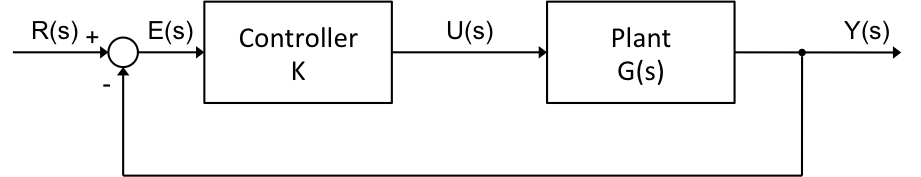
\includegraphics[width=0.8\linewidth]{closed_loop_diagram}
 		\end{figure}
 		Solve by using direct calculations of the root locations.
	\end{example}
\end{frame}

\begin{frame}
	\begin{exampleblock}{}
		\textbf{Solution}: in terms of our notation
		\vspace{-0.5em}
		\begin{columns}
			\begin{column}{0.2\textwidth}
				\begin{align*}
				m &=0,\\
				n &=2,
				\end{align*}
			\end{column}
			\begin{column}{0.2\textwidth}
				\begin{align*}
				K_G =1,\\
				K_A =K,
				\end{align*}
			\end{column}
			\begin{column}{0.2\textwidth}
				\begin{align*}
				b(s) =1,\\
				a(s) = s(s+1).
				\end{align*}
			\end{column}
		\end{columns}
		\vspace{1em}
		We can use the root-locus form $a(s) + Kb(s) = 0$ to obtain a quadratic equation of which the roots will produce a graph.\\ 
		In this case, the quadratic equation is:
		\begin{equation}
		s^2 + s + K = 0
		\end{equation}
		has roots:
		\begin{equation}
		r_1,r_2 = -\frac{1}{2} \pm \frac{\sqrt{1 - 4K}}{2}.
		\end{equation}
	\end{exampleblock}
\end{frame}

\begin{frame}
	\begin{exampleblock}{}
		The root locus is shown below
		\begin{figure}
			\centering
			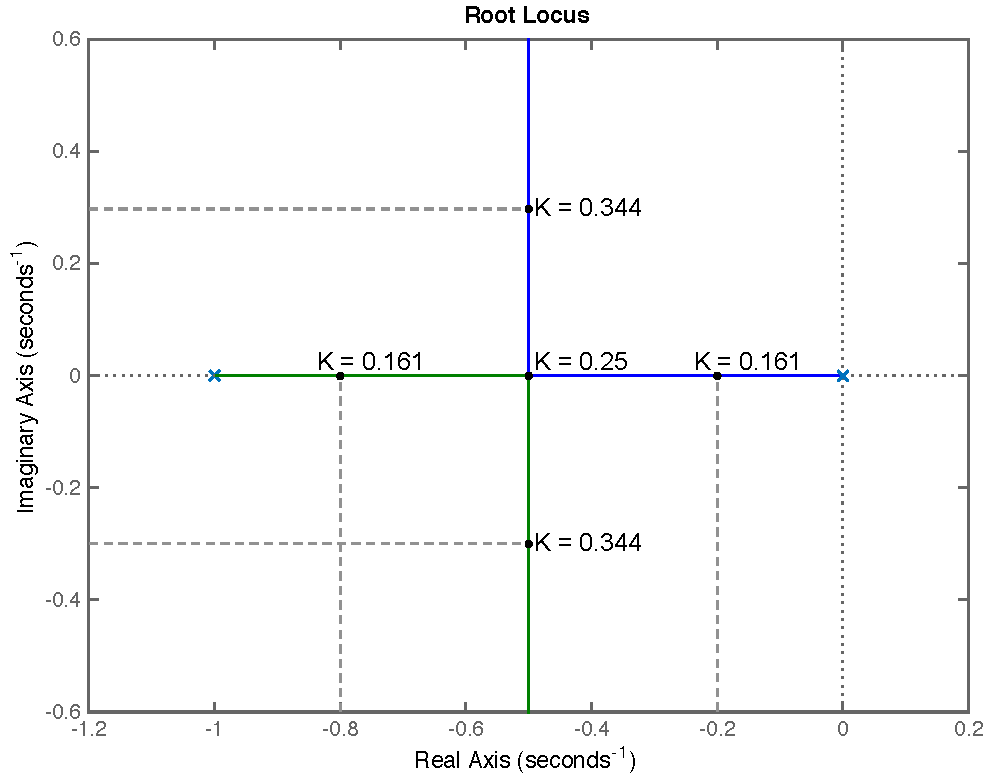
\includegraphics[width=0.7\linewidth]{root_locus_ex1}
		\end{figure}
	\end{exampleblock}
\end{frame}

\begin{frame}
	\begin{exampleblock}{}
		\begin{itemize}
		\item For $0\leq K \leq \frac{1}{4}$, the roots are real between $-1$ and $0$;
		\item At $K = \frac{1}{4}$ there are two roots at $-\frac{1}{2}$;
		\item For $K>\frac{1}{4}$ the roots become complex, with a real part of $-\frac{1}{2}$ and an imaginary part that increases essentially in proportion to the square root of K.
		\end{itemize}
	\end{exampleblock}
\end{frame}

\section{How To Sketch the Root Locus}

\subsection{General Approach}

\begin{frame}
\frametitle{General approach}
	Now look at the equation: $G(s) = -\frac{1}{K}$. If $K$ is to be real and positive, $G(s)$ must be real and negative. This means that if we arrange G(s) in polar form as magnitude and phase, $G(s)$ must have the opposite phase of $K$ in order to satisfy the equation above. We can thus define a root locus in terms of this phase condition:  
	\vspace{0.5em}
	\begin{block}{Definition II}
		The root locus of $G(s)$ is the set of points in the s-plane where the phase of $G(s)$ is $180^{\circ}$.	
	\end{block}
\end{frame}

\begin{frame}
\frametitle{General approach}
	Since the phase remains unchanged if an integral multiple of $360^{\circ}$ is added, we can express Definition II as: $\angle G(s) = 180^{\circ} + 360^{\circ}l$, where $l$ is any integer. While it is very difficult to solve a high-order polynomial, computing the phase is relatively easy.\\
	\vspace{1em}
	The usual case is when $K$ is real and positive; we call this case the \textbf{positive or $180^{\circ}$ locus}. When $K$ is real and negative, $G(s)$ must be real and positive of $s$ to be on the locus. Therefore, the phase of $G(s)$ must be $0^{\circ}$. This special case is called a \textbf{negative or $0^{\circ}$ locus}.\\
	\vspace{1em}
	Although measuring the phase is easy, measuring the phase at every point in the $s$-plane is hardly practical. It would be better if there would exist some general guidelines we can use for determining where the root locus is situated.
\end{frame}

\begin{frame}
\frametitle{Guidelines in practice}
	We will now sketch the root locus of a system with transfer function:\\
	\begin{exampleblock}{}
		\begin{equation}
		G(s) = \frac{1}{s[(s+4)^{2} + 16]}
		\end{equation}
	\end{exampleblock}
	Using Definition II, we can check whether a point $s_0$ lies on the root locus for some value of $K$ by checking if the following expression is valid: 
	\begin{exampleblock}{}
		\begin{equation}
		\angle 1 - \angle s_0 -\angle [(s_0 + 4)^2 + 16] = 180^{\circ} + 360^{\circ}l
		\end{equation}
	\end{exampleblock}
	but as already mentioned, it is not practical to do this for every point. So we will now use the general guidelines to sketch the root locus. 
\end{frame}	

\begin{frame}
\frametitle{STEP 1: the open-loop $\times's$ and $\circ's$}
	Calculate and plot the open-loop poles and zero's:
	\begin{exampleblock}{}
		\begin{figure}
			\centering
			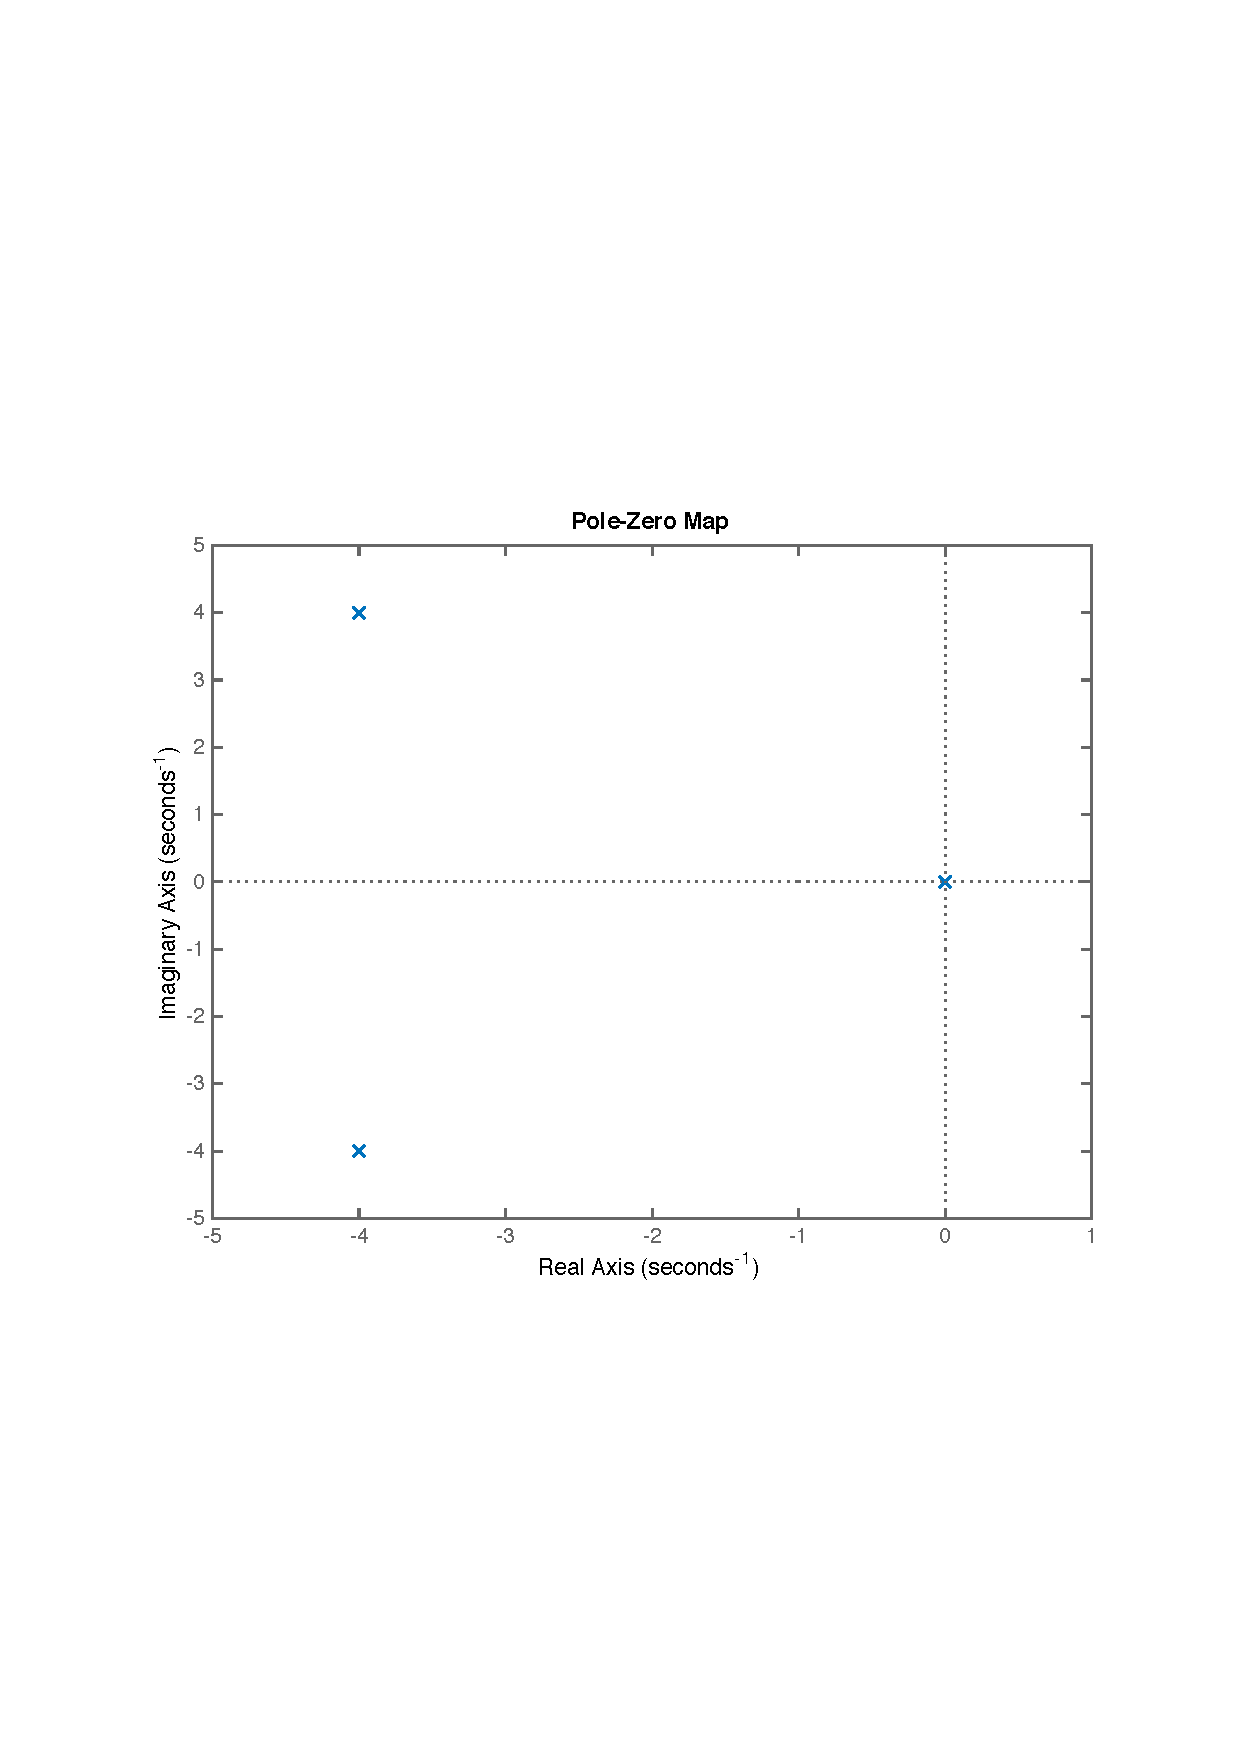
\includegraphics[width=0.6\linewidth]{how_to_draw_ex1}
		\end{figure}
	\end{exampleblock}
\end{frame}

\begin{frame}
\frametitle{STEP 2: locus on real axis}
	The portion of the real axis to the left of an odd number (counted from the right) of open loop poles and zeros are part of the locus:
	\begin{exampleblock}{}
		\begin{figure}
			\centering
			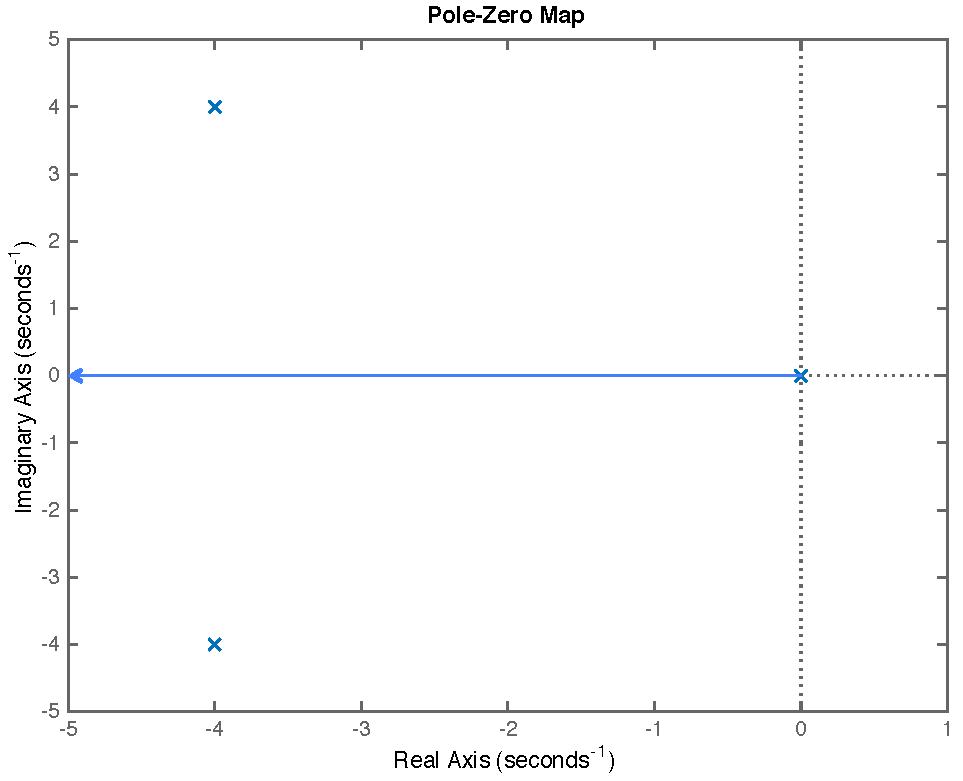
\includegraphics[width=0.6\linewidth]{how_to_draw_ex2}
		\end{figure}
	\end{exampleblock}
\end{frame}

\begin{frame}
\frametitle{STEP 3: asymptotes for large values of K}
	As K approaches $\infty$, the equation $G(s) = -\frac{1}{K}$ can be satisfied only if $G(s) = 0$ where $G(s) = \frac{b(s)}{a(s)}$.\\
	\vspace{1em}
	We can now substitute this in $1 + KG(s) = 0$, resulting in the following equation:
	\begin{equation}
	1 + K\frac{b(s)}{a(s)} = 1 + K\frac{s^m + b_1s^{m-1} + ... + b_m}{s^n + a_1s^{n-1} + ... + a_n} = 0
	\end{equation}
	Since $n < m$, $G(s) = 0$ can occur when: 
	\begin{itemize}
		\item $b(s) = 0$;
		\item $s \rightarrow \infty$.
	\end{itemize}
\end{frame}

\begin{frame}
\frametitle{STEP 3: asymptotes for large values of K}
	We now look closer to the second condition: $G(s) = 0$ when $s \rightarrow \infty$.\\
	\vspace{1em}
	For very large values of $s$, the highest-order power of $s$ in Eq.(8) predominates. We can divide $a(s)$ by $b(s)$ and match the dominant two terms (highest powers in $s$) to the expansion $(s-\alpha)^{n-m}$, resulting in the following approximation:
	\begin{equation}
		1 + K\frac{1}{(s-\alpha)^{n-m}}
	\end{equation}
	We need to find the locus for the asymptotic system (Eq.(8)) and $\alpha$.
\end{frame}

\begin{frame}	
\frametitle{STEP 3: asymptotes for large values of K}
	To find the locus, we choose $s_0 = Re^{j\phi}$ for some large value of $R$ and some variable $\phi$.\\
	\vspace{1em}
	Since all poles of Eq.(9) are in the same place, the angle of its transfer function is $180^{\circ}$ if all $n-m$ angles ($\phi_l$) sum to $180^{\circ}$. Therefore, $\phi_l$ is given by: 
	\begin{equation}
	\phi_l = \frac{180^{\circ} + 360^{\circ}l}{n-m}, l = 1,2,...,n-m
	\end{equation}	
	\vspace{-0.5em}	
	\begin{exampleblock}{}
	For our system: $n-m=3$, thus $\phi_1, \phi_2, \phi_3 = 60^{\circ}, 180^{\circ}, 300^{\circ}$.
	All the lines of the asymptotic locus come from $s_0 = \alpha$.
	\end{exampleblock}
\end{frame}

\begin{frame}
\frametitle{STEP 3: asymptotes for large values of K}
	To determine $\alpha$ we use a simple property of polynomials. Suppose we have a monic polynomial with coefficients $a_i$ and roots $p_i$ and we equate the polynomial form with the factored form:
	\begin{center}
		$s^n + a_1s^{n-1} + a_2s^{n-2} + ... + a_n = (s-p_1)(s-p_2)...(s-p_n).$
	\end{center}
	If we multiply out the factors on the right side of this equation, we can see that the coefficient of $s^{n-1}$ is $-p_1 - p_2 - ... - p_n$. On the left side of the equation we see that this term is $a_1$.\\
	\vspace{1em}
	Consequently $a_1 = -\Sigma p_i$, the coefficient of the second-highest term in a monic polynomial is the negative sum of its roots (the poles of $G(s)$). The same can be concluded for $b_1 = -\Sigma z_i$.
\end{frame}

\begin{frame}
\frametitle{STEP 3: asymptotes for large values of K}
	Applying these results in the closed-loop characteristic polynomial, leads to:
	\begin{center}
		$s^n + a_1 s^{n-1} + ... + a_n + K(s^m + b_1 s^{m-1} + ... + b_m) = 0$.
	\end{center}
	The negative of the sum of the poles is the coefficient of $s^{n-1}$ and is independent of $K$ if $m < n-1$. However, since this is the closed-loop characteristic equation, this coefficient is the negative of the sum of the roots of the closed-loop system $\Sigma r_i$, hence
	\begin{itemize}
		\item the center point of the roots does not change with $K$ if $m < n-1$;
		\item $-\Sigma r_i = -\Sigma p_i$.
	\end{itemize}
\end{frame}

\begin{frame}
\frametitle{STEP 3: asymptotes for large values of K}
	For large values of $K$, $m$ of the roots $r_i$ are approximately equal to the zeros $z_i$ and $n-m$ of the roots are from the asymptotic $\frac{1}{(s-\alpha)^{n-m}}$ system, whose poles add up to $(n-m)\alpha$.\\
	\vspace{1em}
	Combining these results we conclude that the sum of all the roots equals the sum of those roots that go to infinity plus the sum of those roots that go to the zeros of $G(s)$:
	\begin{center}
		$+\Sigma r_i = + (n-m)\alpha + \Sigma z_i = +\Sigma p_i$.
	\end{center}
	Solving for $\alpha$ we get 
	\begin{center}
		$\alpha = \frac{\Sigma p_i - \Sigma z_i}{n-m}$.
	\end{center}
\end{frame}

\begin{frame}
\frametitle{STEP 3: asymptotes for large values of K}
	Complex poles and zeros always occur in complex conjugate pairs, consequently in the sums $\Sigma p_i$ and $\Sigma z_i$ the imaginary parts will always add to zero.\\
	\vspace{0.5em}
	\begin{exampleblock}{}
	For our system: $\alpha = \frac{-4-4+0}{3-0} = -2.67.$\\
	\vspace{1em}
	We can now use the results for $\phi_1, \phi_2, \phi_3$ and $\alpha$ to draw the asymptotes. 
	\end{exampleblock}
\end{frame}

\begin{frame}
\frametitle{STEP 3: asymptotes for large values of K}
	\begin{exampleblock}{}
		\begin{figure}
			\centering
			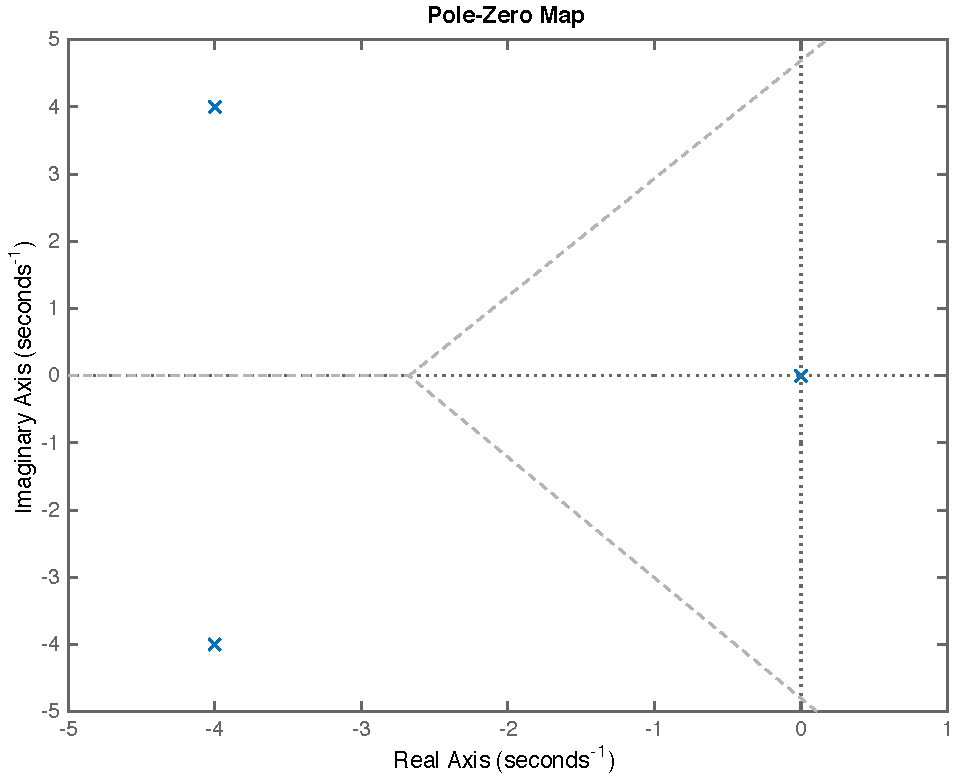
\includegraphics[width=0.7\linewidth]{how_to_draw_ex3}
		\end{figure}
	\end{exampleblock}
\end{frame}

\begin{frame}
\frametitle{STEP 4: departure and arrival angles}
	We know that the locus begins at the $\times's$ and that it goes to either $\circ's$ or to infinity along the radial asymptotic lines.\\
	\vspace{1em}
	We next compute the angle by which a branch of the locus departs from one of the poles. We take a test point $s_0$ very near pole 2 at $-4+4j$ and compute the angle of $G(s_0)$ (illustration see next slide). We select the test point close enough to pole 2 that the angles $\phi_1$ and $\phi_3$ to the test point can be considered the same as those angles to pole 2: $\phi_1 = 90^{\circ}$ and $\phi_3 = 135^{\circ}$. 
\end{frame}

\begin{frame}
\frametitle{STEP 4: departure and arrival angles}
	\begin{figure}
		\centering
		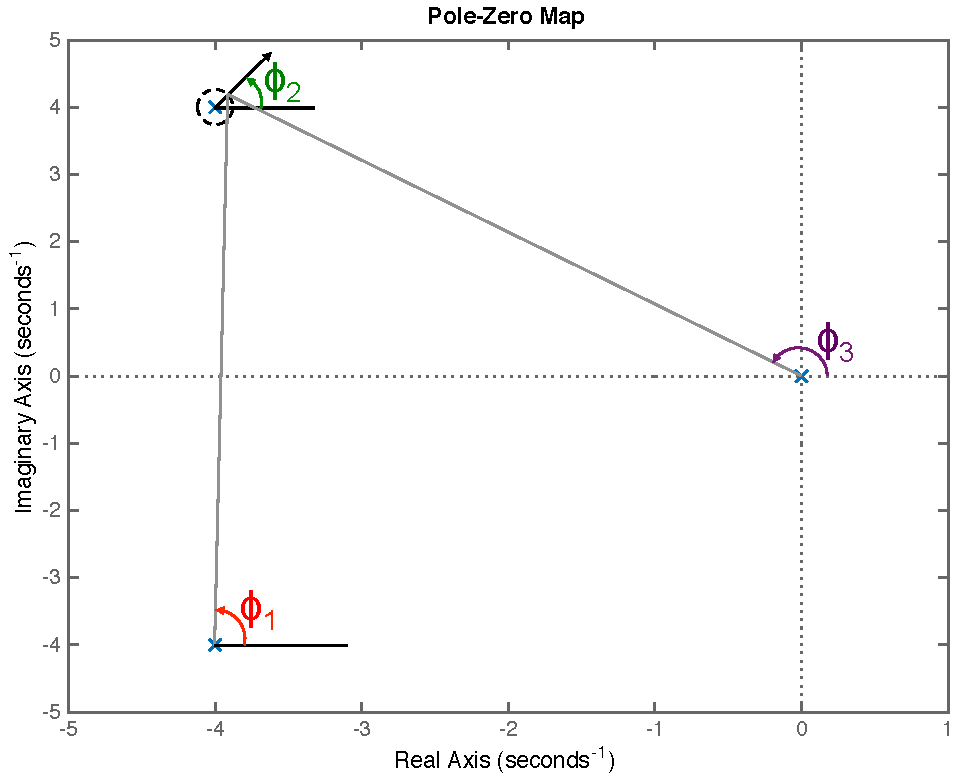
\includegraphics[width=0.7\linewidth]{how_to_draw_ex4}
	\end{figure}
\end{frame}

\begin{frame}
\frametitle{STEP 4: departure and arrival angles}	
	\begin{exampleblock}{}
	We can calculate $\phi_2$ from the angle condition:
	\begin{center}
		$-90^{\circ} - \phi_2 - 135^{\circ} = +180^{\circ} + 360^{\circ}l$
	\end{center}
	where $l$ is chosen so that $-180^{\circ} < \phi_2 < +180^{\circ}$. If we take $l = -1$, then $\phi_2 = -45^{\circ}$.\\
	\vspace{1em}
	By the complex conjugate symmetry of the plots, the angle of departure of the locus near pole 1 at $-4 - 4j$ will be $+45^{\circ}$. The angle of departure from pole 3 at the origin is $180^{\circ}$.
	\end{exampleblock}
\end{frame}

\begin{frame}
\frametitle{STEP 4: departure and arrival angles}	
	\begin{exampleblock}{}
		\begin{figure}
			\centering
			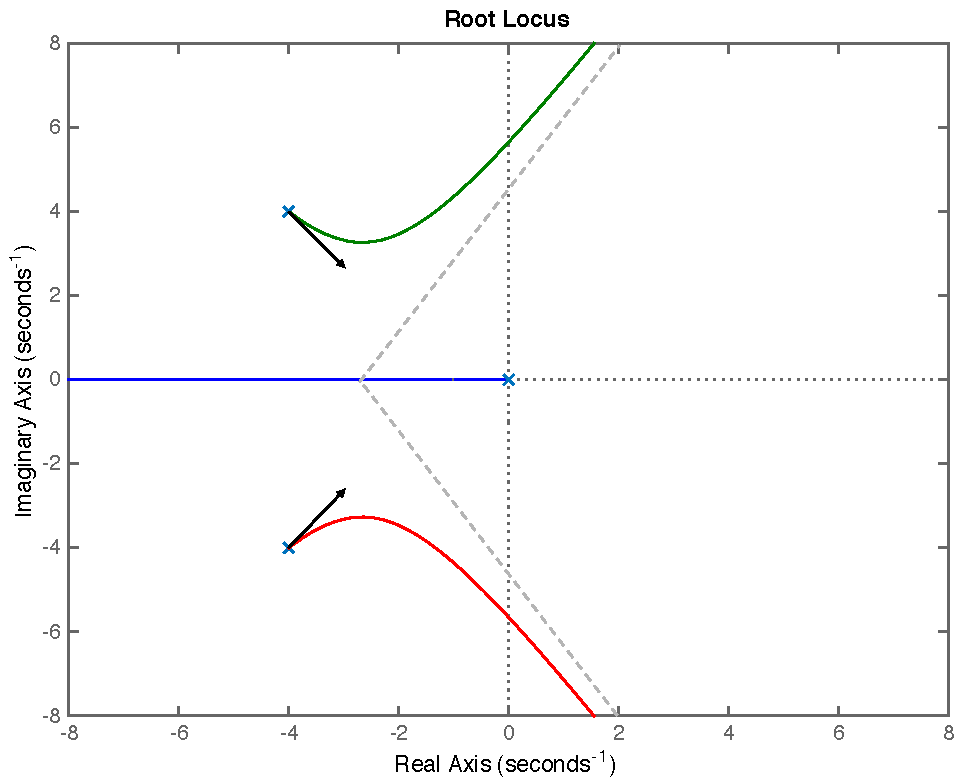
\includegraphics[width=0.7\linewidth]{how_to_draw_ex5}
		\end{figure}
	\end{exampleblock}
\end{frame}

\begin{frame}
\frametitle{STEP 5: location of multiple roots and their arrival and departure angles}
	\begin{itemize}
	\item Two locus segments coming together at any point in the s-plane will always approach at at relative angle of $180^{\circ}$ and then break away with a $90^{\circ}$ change in direction; 
	\item Three locus segments coming together will always approach at $120^{\circ}$ angles that are rotated $60^{\circ}$ relative to the arrival angles.
	\end{itemize}
	\begin{exampleblock}{}
		In our example, this step is not applied. But the first case (with two locus segments) can be seen in the first example from this chapter. 
	\end{exampleblock}
\end{frame}

\begin{frame}
\frametitle{STEP 6: Complete the sketch}
	\begin{exampleblock}{}	
		\begin{figure}
			\centering
			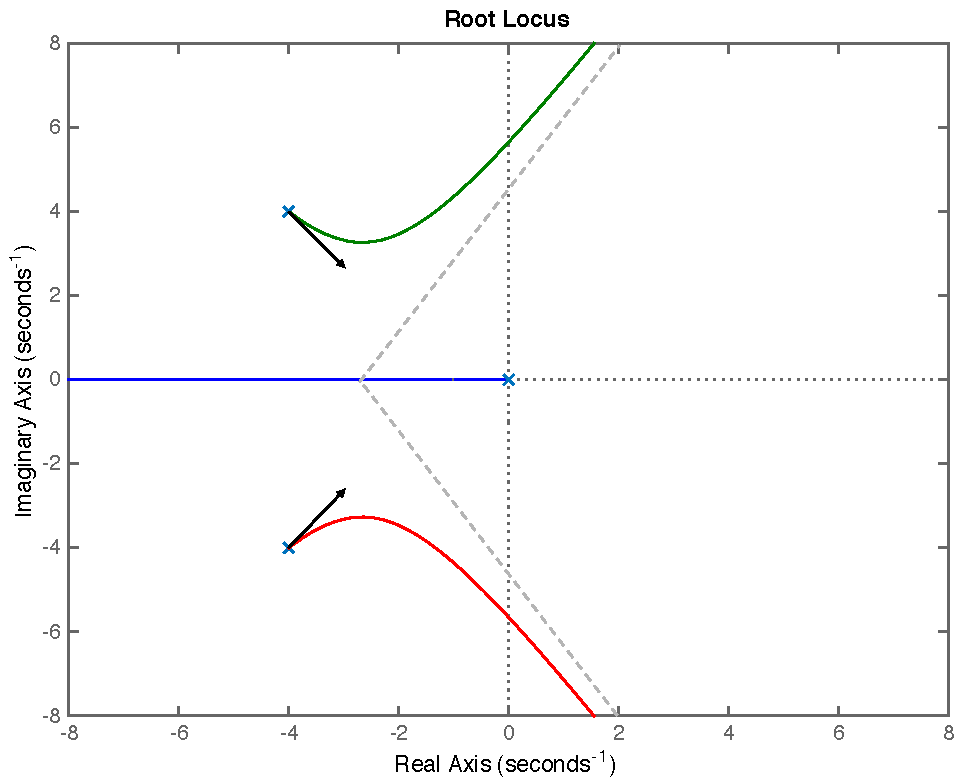
\includegraphics[width=0.7\linewidth]{how_to_draw_ex6}
		\end{figure}
	\end{exampleblock}
\end{frame}

\subsection{Rules of thumb for sketching the root locus}

\begin{frame}
	\frametitle{Overview of the guidelines}
	\begin{block}{}
		Drawing the root locus yourself can be done by following the next steps:
		\vspace{0.5em}
		\begin{enumerate}
			\item Mark poles with $\times$ and zeros with $\circ$;
			\item Draw the locus on the real axis to the left of an odd number of real poles plus zeros;
			\item Draw the asymptotes, centered at $\alpha$ and leaving at angles $\phi_l$, where:
			\vspace{-0.5em}
			\begin{align*}
			n - m &=  \# asymptotes\\
			\alpha &= \frac{\varSigma p_i - \varSigma z_i}{n-m}\\
			\phi_l &= \frac{180^{\circ} + 360^{\circ}(l - 1)}{n - m}, l = 1,2,...,n-m.
			\end{align*}
		\end{enumerate}
	\end{block}
\end{frame}

\begin{frame}
	\frametitle{Overview of the guidelines}
	\begin{block}{}
		\begin{enumerate}
			\setcounter{enumi}{3}
			\item Compute locus departure angles from te poles and arrival angles at the zeros:
			\begin{align*}
			q\phi_{dep} &= \varSigma\psi_i - \varSigma\phi_i - 180^{\circ} - 360^{\circ}l,\\
			q\psi_{arr} &= \varSigma\phi_i - \varSigma\psi_i + 180^{\circ} + 360^{\circ}l,
			\end{align*}
			where $q$ is the multiplicity of the pole or zero and $l$ takes on $q$ integer values so that the angles are between $\pm180^{\circ}$. $\Sigma \phi_i$ is the sum of the angles of the (remaining) poles and $\Sigma \psi_i$ is the sum of the angles of the (remaining) zeros.
		\end{enumerate}
	\end{block}
\end{frame}

\begin{frame}
	\frametitle{Overview of the guidelines}
	\begin{block}{}
		\begin{enumerate}
			\setcounter{enumi}{4}
			\item Use the results from the study of multiple roots to help in sketching how locus segments come together and break away: two segments come together at $180^{\circ}$ and break away at $\pm 90^{\circ}$, three locus segments approach each other at relative angles of $120^{\circ}$ and depart at angles rotated by $60^{\circ}$.
			\item Complete the locus, using the facts developed in the previous steps and making reference to the illustrative loci for guidance. The locus branches start at poles and at zeros or infinity.
		\end{enumerate}
	\end{block}
		If further refinement is required at the stability boundary, you can also estimate the points where the root locus crosses the imaginary axis. This is done by using Routh's stability criterion. We don't discuss it in this course, but you can find an explanation for it in the additional material of this chapter.  
\end{frame}

\begin{frame}
\frametitle{Important to remember!}
	\begin{alertblock}{}
		While you are sketching your root locus, keep the following things in mind:
		\begin{enumerate}
			\item The root locus hax max($\#$poles of $G(s)$, $\#$ zeros of $G(s)$) branches;
			\item Complex roots of $1 + KG(s)$ (closed loop poles) always occur in conjugate pairs;
			\item A branch will never cross over itself;
			\item Branches leave and enter the real axis at $90^{\circ}$ (this is not a $100\%$ general rule, but it is true in most cases);
		\end{enumerate}
	\end{alertblock}
\end{frame}

\begin{frame}
\frametitle{Important to remember!}
	\begin{alertblock}{}
		\begin{enumerate}
		\setcounter{enumi}{4}
			\item Each branch starts at an open loop pole of $G(s)$ (for $K=0$) and ends at a closed loop zero of $G(s)$ (for $K \rightarrow \infty$). If $\#$poles of $G(s)$ $\neq$ $\#$zeros of $G(s)$ the extra branches go to/come from a zero/pole in infinity.
		\end{enumerate}
	\vspace{-1em}
	\begin{columns}
		\begin{column}{0.5\textwidth}
			\begin{figure}
				\centering
				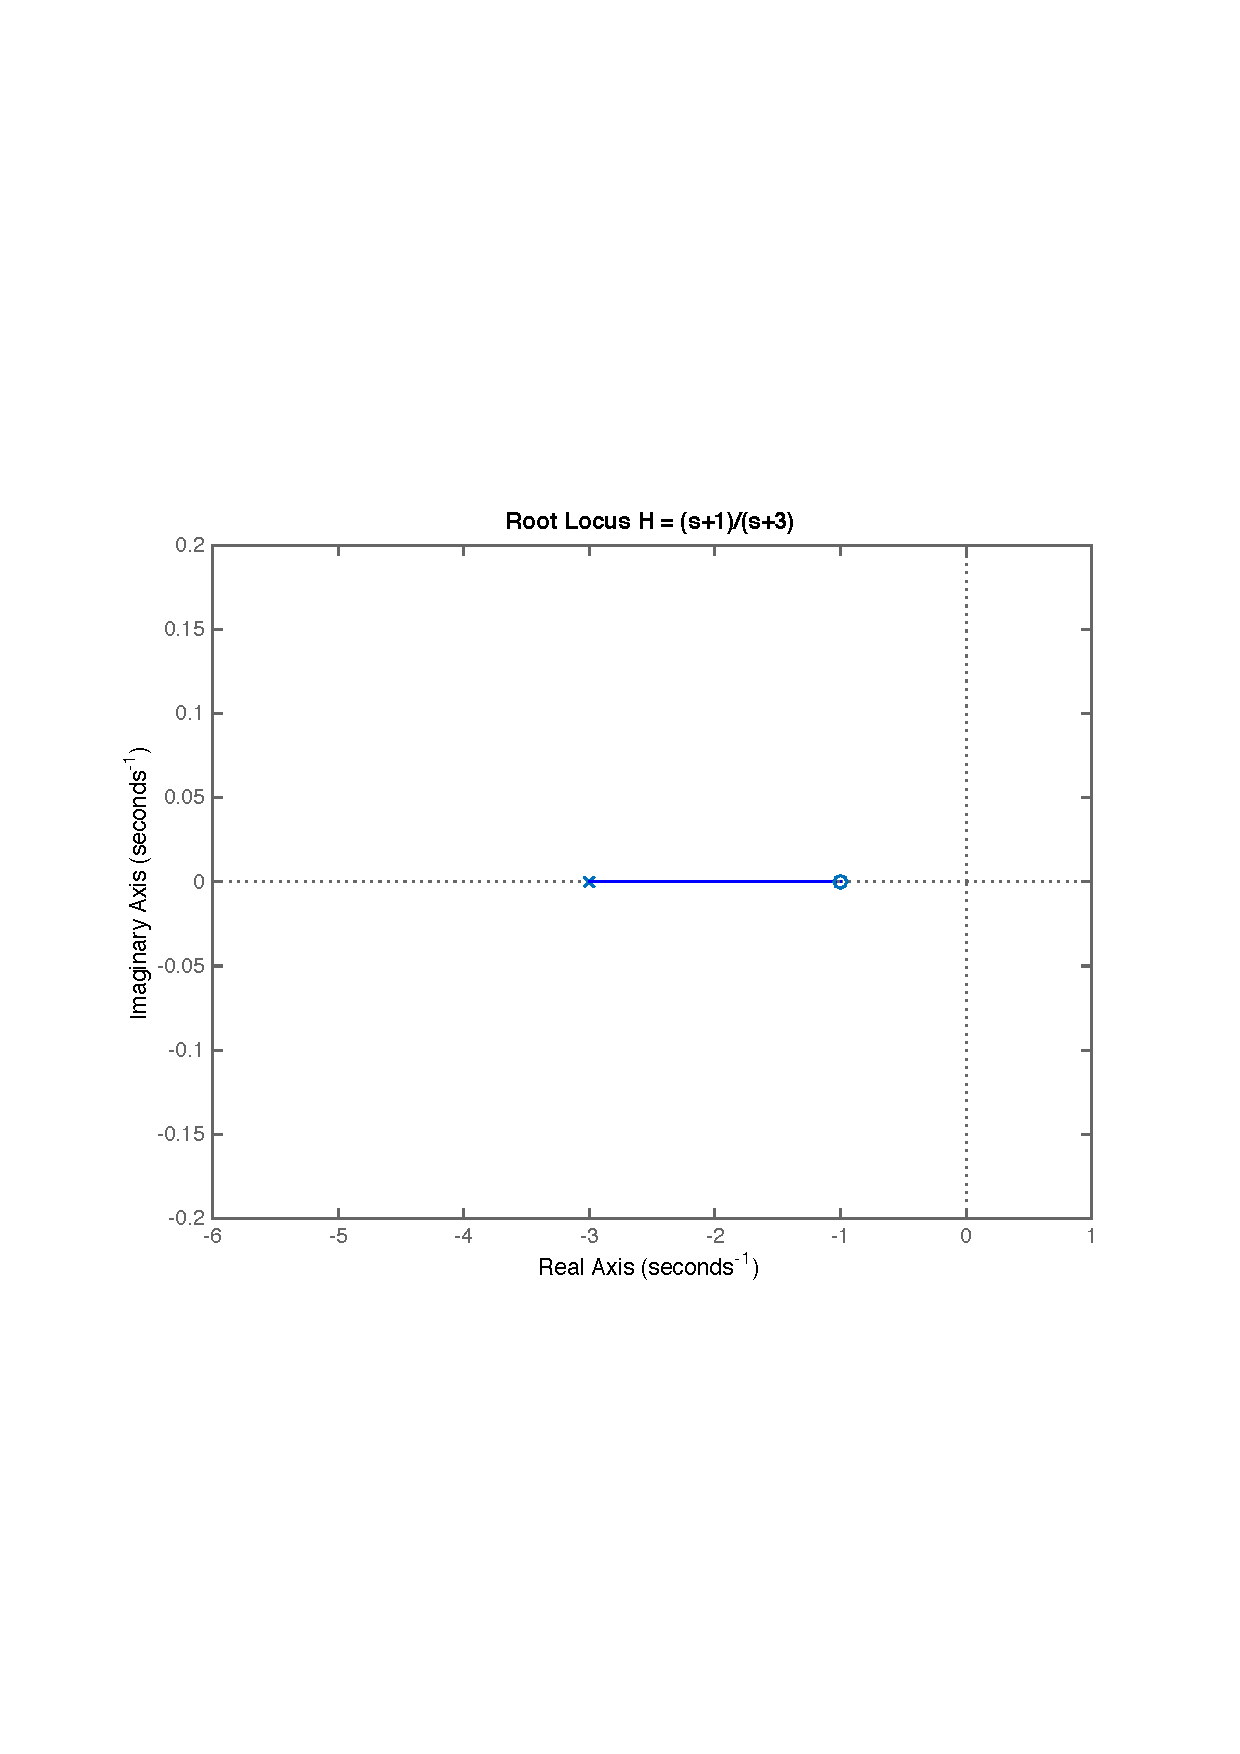
\includegraphics[width=0.8\linewidth]{how_to_draw_easy_ex1}
			\end{figure}
		\end{column}
		\begin{column}{0.5\textwidth}
			\begin{figure}
				\centering
				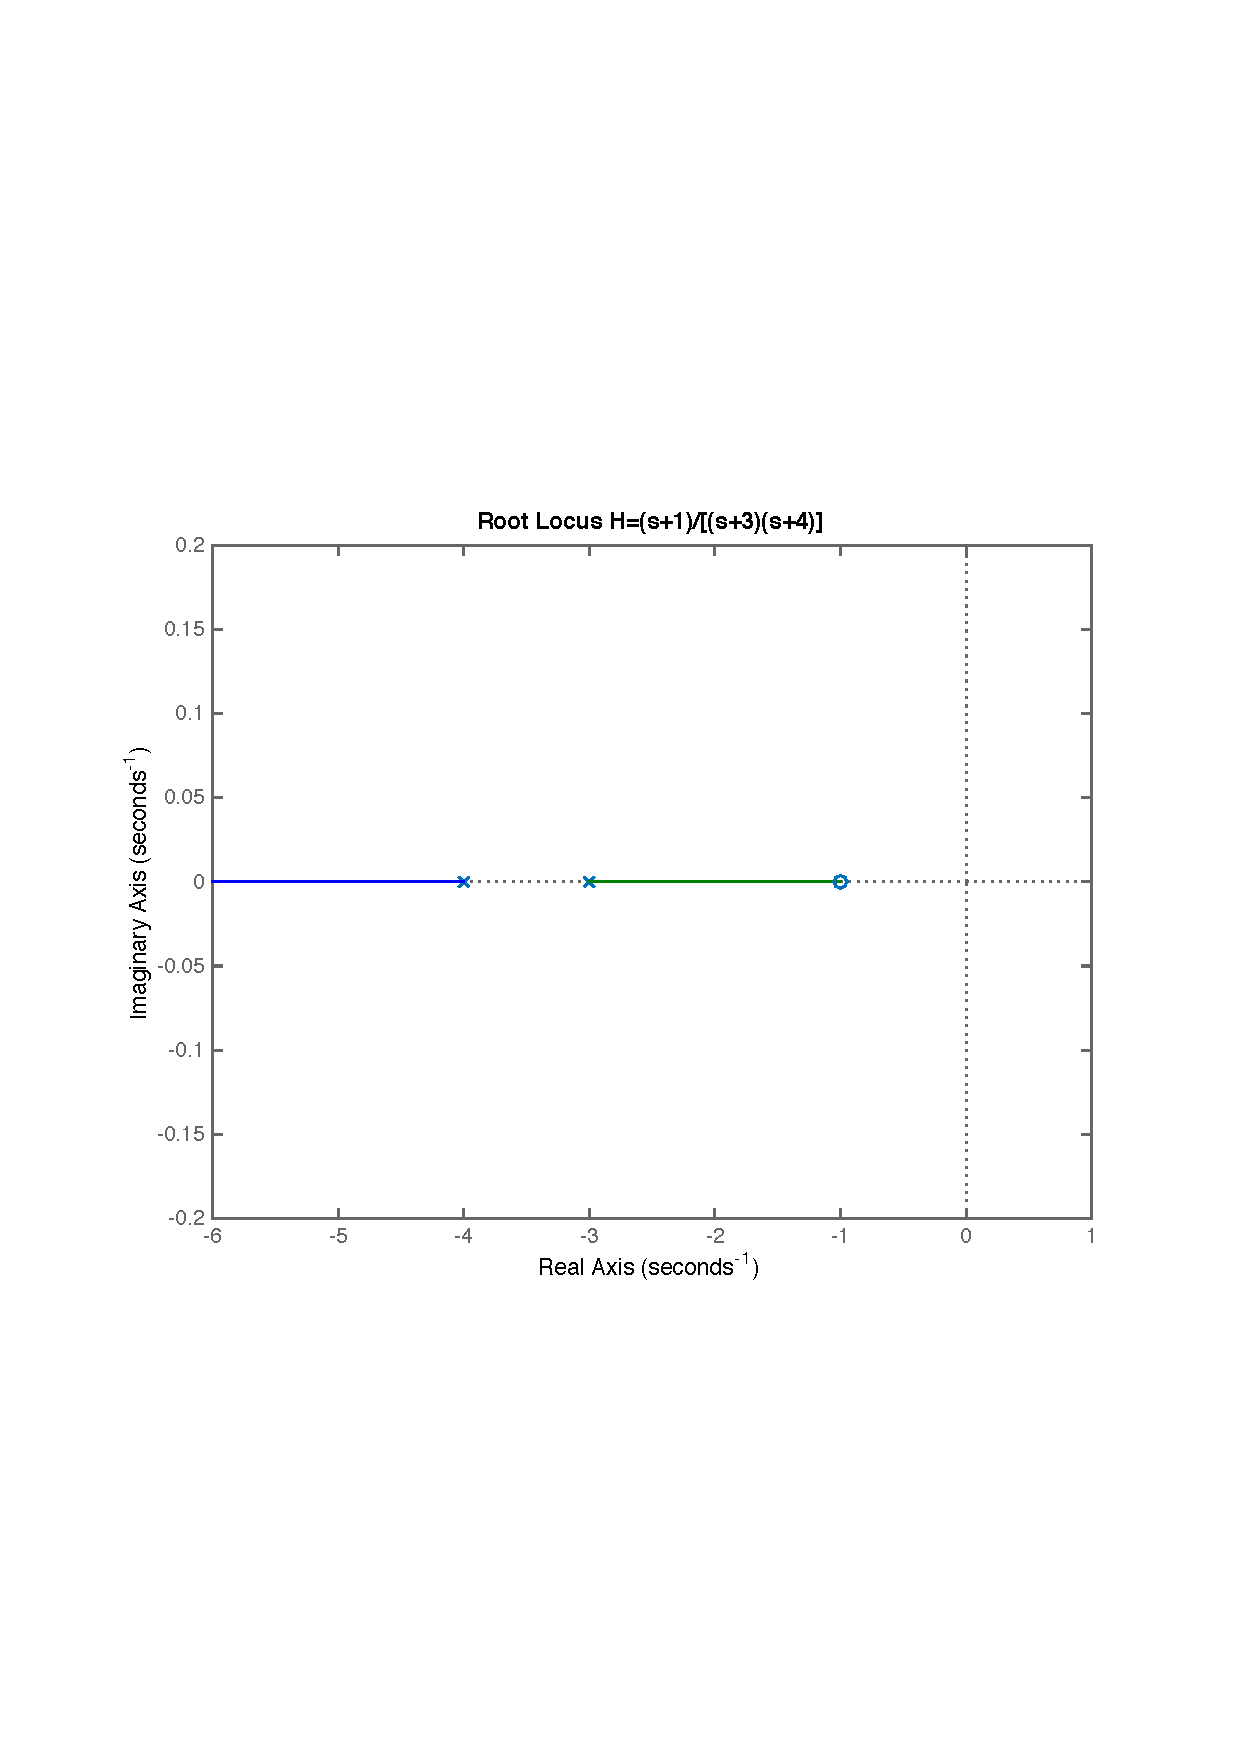
\includegraphics[width=0.8\linewidth]{how_to_draw_easy_ex2}
			\end{figure}
		\end{column}
	\end{columns}
	\end{alertblock}
\end{frame}

\begin{frame}
	\frametitle{Example 1}
	\begin{example}
		Try to understand why the root locus of the following system, $H(s) = \frac{(s + 0.2)(s + 1)}{s(s + 0.8)(s - 1)}$, takes the shape as shown in the figure.
		\begin{figure}
			\centering
			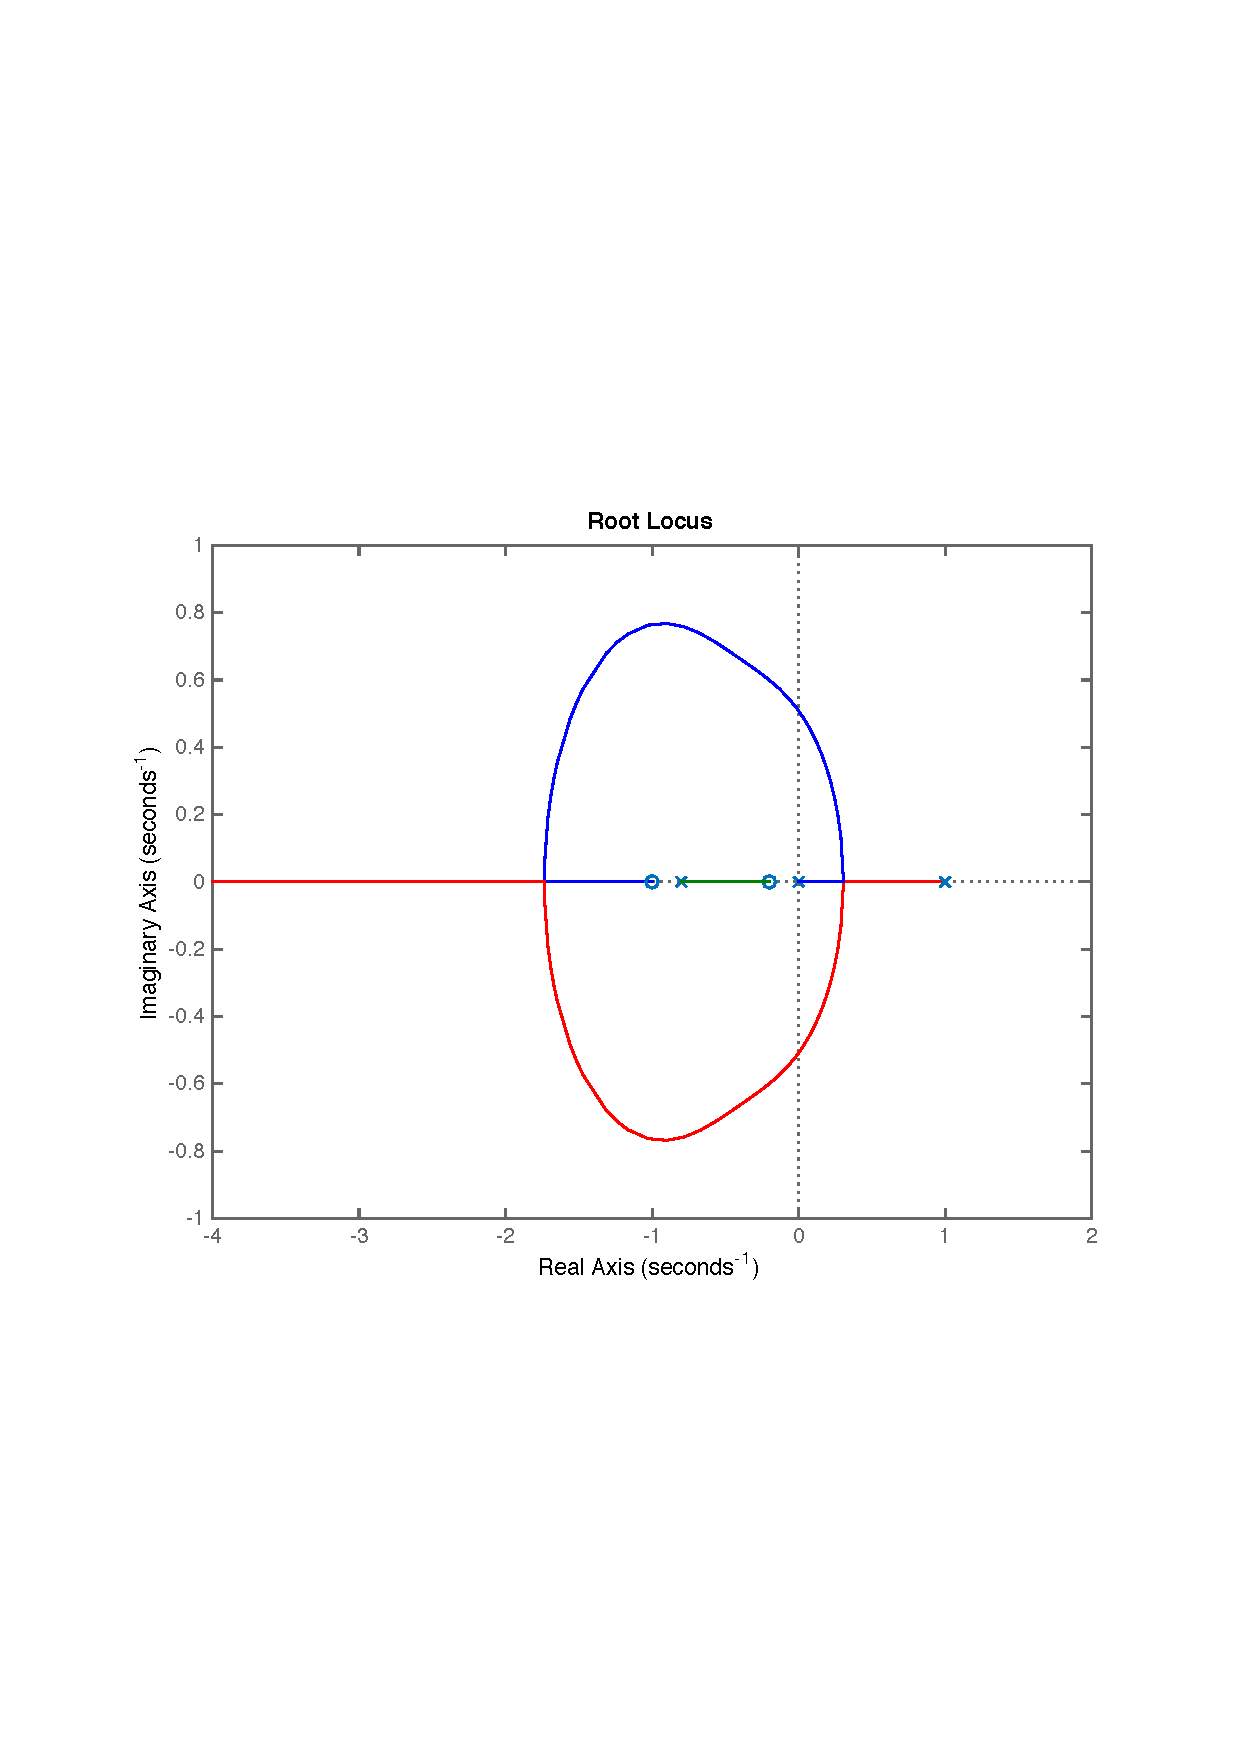
\includegraphics[width=0.5\linewidth]{simple_ex1}
		\end{figure}
	\end{example}
\end{frame}

\section{Design criteria}

\begin{frame}
\frametitle{Second order system}
	Recall from chapter 5 that the dynamic behavior of the second-order system can be described in terms of only two parameters $\zeta$ and $\omega_n$.
	\vspace{-1em}
	\begin{figure}
		\centering
		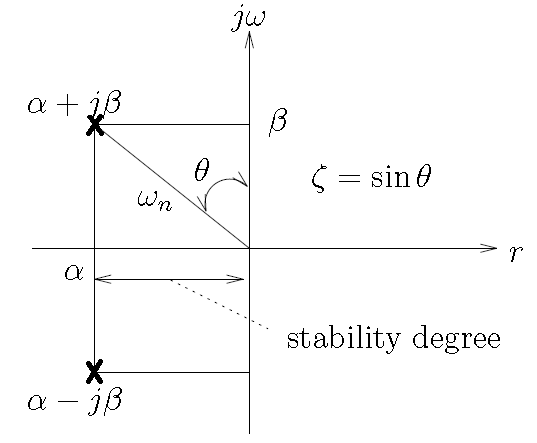
\includegraphics[width=0.6\linewidth]{poles_system}
	\end{figure}
\end{frame}

\begin{frame}
\frametitle{Root locus method: design criteria}
	If you are able to express your design criteria in terms of the poles ($\alpha + j\beta$, with $\alpha < 0$ and $\beta>0$), you can find out if there are any $K$-values appropriate and, more importantly, which $K$-values.\\
	\begin{block}{Criteria}
	\begin{itemize}
		\item The damping ratio: $\zeta = \frac{\beta}{\mid \alpha + j\beta\mid}$ ($0 \leq \zeta \leq 1$);
		\item The natural frequency: $\omega_n = -\frac{\alpha}{\zeta} = \frac{\beta}{\sqrt{1 - \zeta^2}}$;
		\item The rise time: $t_r \cong \frac{1.8}{\omega_n}$;
		\item The settling time: $t_s = \frac{4.6}{\zeta \omega_n}$;
		\item The peak time: $t_p =\frac{\pi}{\omega_d}$, with $\omega_d = \omega_n \sqrt{1 - \zeta^2} $;
		\item The overshoot: $M_p = e^{-\pi \frac{\zeta}{\sqrt{1 - \zeta^2}}}$.
	\end{itemize}
	\end{block}
\end{frame}

\begin{frame}
\frametitle{Example design criteria}
	\begin{example}
		We will now apply a design criteria on a system from a previous example which we discussed in the first subsection:
		\vspace{-0.5em}
		\begin{equation}
		G(s) = \frac{1}{s(s+1)}.
		\vspace{-0.5em}
		\end{equation}
		We can now compute K at the point where the locus crosses $\zeta = 0.5$: we know that if $\zeta = 0.5$, then $\theta = 30^{\circ}$ and the magnitude of the imaginary part of the root is $\sqrt{3}$ times the magnitude of the real part. The magnitude of the real part is $\frac{1}{2}$ and thus, we have:
		\vspace{-0.5em}
		\begin{equation}
		\frac{\sqrt{4K - 1}}{2} = \frac{\sqrt{3}}{2}
		\vspace{-0.5em}
		\end{equation}
		and therefore, $K = 1$.
	\end{example}
\end{frame}

\begin{frame}
\frametitle{Root locus method: design criteria}
	The possible design criteria for second order systems are very useful since they represent physically important measures in terms of the poles.\\
	\begin{alertblock}{Second order approximation}
		For most of the time only one or two poles dominate the behavior of the system. These are called the dominant poles. Consequently many systems behave more or less as if they are of second order. 
	\end{alertblock}
	\begin{itemize}
		\item A single pole at position $-a$ results in a $e^{-at}$ term in the output. So after some time, the poles with the largest real part will dominate the behavior;
		\item A single pole at position $me^{j\omega}$ results in a $m^ke^{j\omega k}$ term in the output. So after some time the poles with the largest modulus will dominate. 
	\end{itemize}
\end{frame}
	
\section{Root Locus and MATLAB}

\subsection{Root Locus}

\begin{frame}
\frametitle{MATLAB Commands}
	MATLAB provides a function to plot the root locus and the zero-pole map of a system:
	\begin{itemize}
		\item root locus: \textbf{"rlocus(sys)"}
		\item zero pole: \textbf{"pzmap(sys)"}
	\end{itemize} 
	\vspace{1em}
	Most of the time you want to use the plot of the root locus to decide which value of $K$ you need to satisfy the requirements. To visualize these requirement, you can use the command \textbf{"sgrid(requirement1, requirement2,...)"}. This will result in a grid that envisions the requirements.\\
	\vspace{1em}
	You can also just include a grid (\textbf{"grid"}) in your root locus plot which can help you locate the poles.
\end{frame}

\begin{frame}
\frametitle{MATLAB Commands}
	You can choose the desired poles on the locus in MATLAB by using the \textbf{"rlocfind(sys)"}-command. This will allow you to select a point on your root locus plot. MATLAB will tell you the precise point you selected, will tell you what the gain is at that point and will tell you the poles of the system with that gain.\\
	\vspace{1em}
	MATLAB can also calculate the closed-loop transfer function. You can do this by using the \textbf{"feedback(K*sys,1)"} command. You only need to specify the value of $K$ if you haven't yet used the \textbf{"rlocfind"} command.
\end{frame}

\begin{frame}
	\begin{example}
		We will now design a controller using MATLAB, the system has the following transfer function: $H(s) = \frac{s+7}{s(s+5)(s+15)(s+20)}$\\
		and must meet the following design criteria: 
		\begin{itemize}
			\item overshoot must be less than $5\%$;
			\item rise time = $1s$
		\end{itemize}
		MATLAB commands:\\
		s = tf ('s') \\
		H = (s+7)/(s*(s+5)*(s+15)*(s+20)) \textcolor{gray}{we define the system H by its transfer function} \\
		rlocus(H) \textcolor{gray}{we command MATLAB to draw the root locus} \\
		axis([-22 3 15 15])	\textcolor{gray}{we adjust the axis} \\
	\end{example}
\end{frame}

\begin{frame}
	\begin{exampleblock}{}
		Which results in the following plot:
		\vspace{-0.5em}
		\begin{figure}
			\centering
			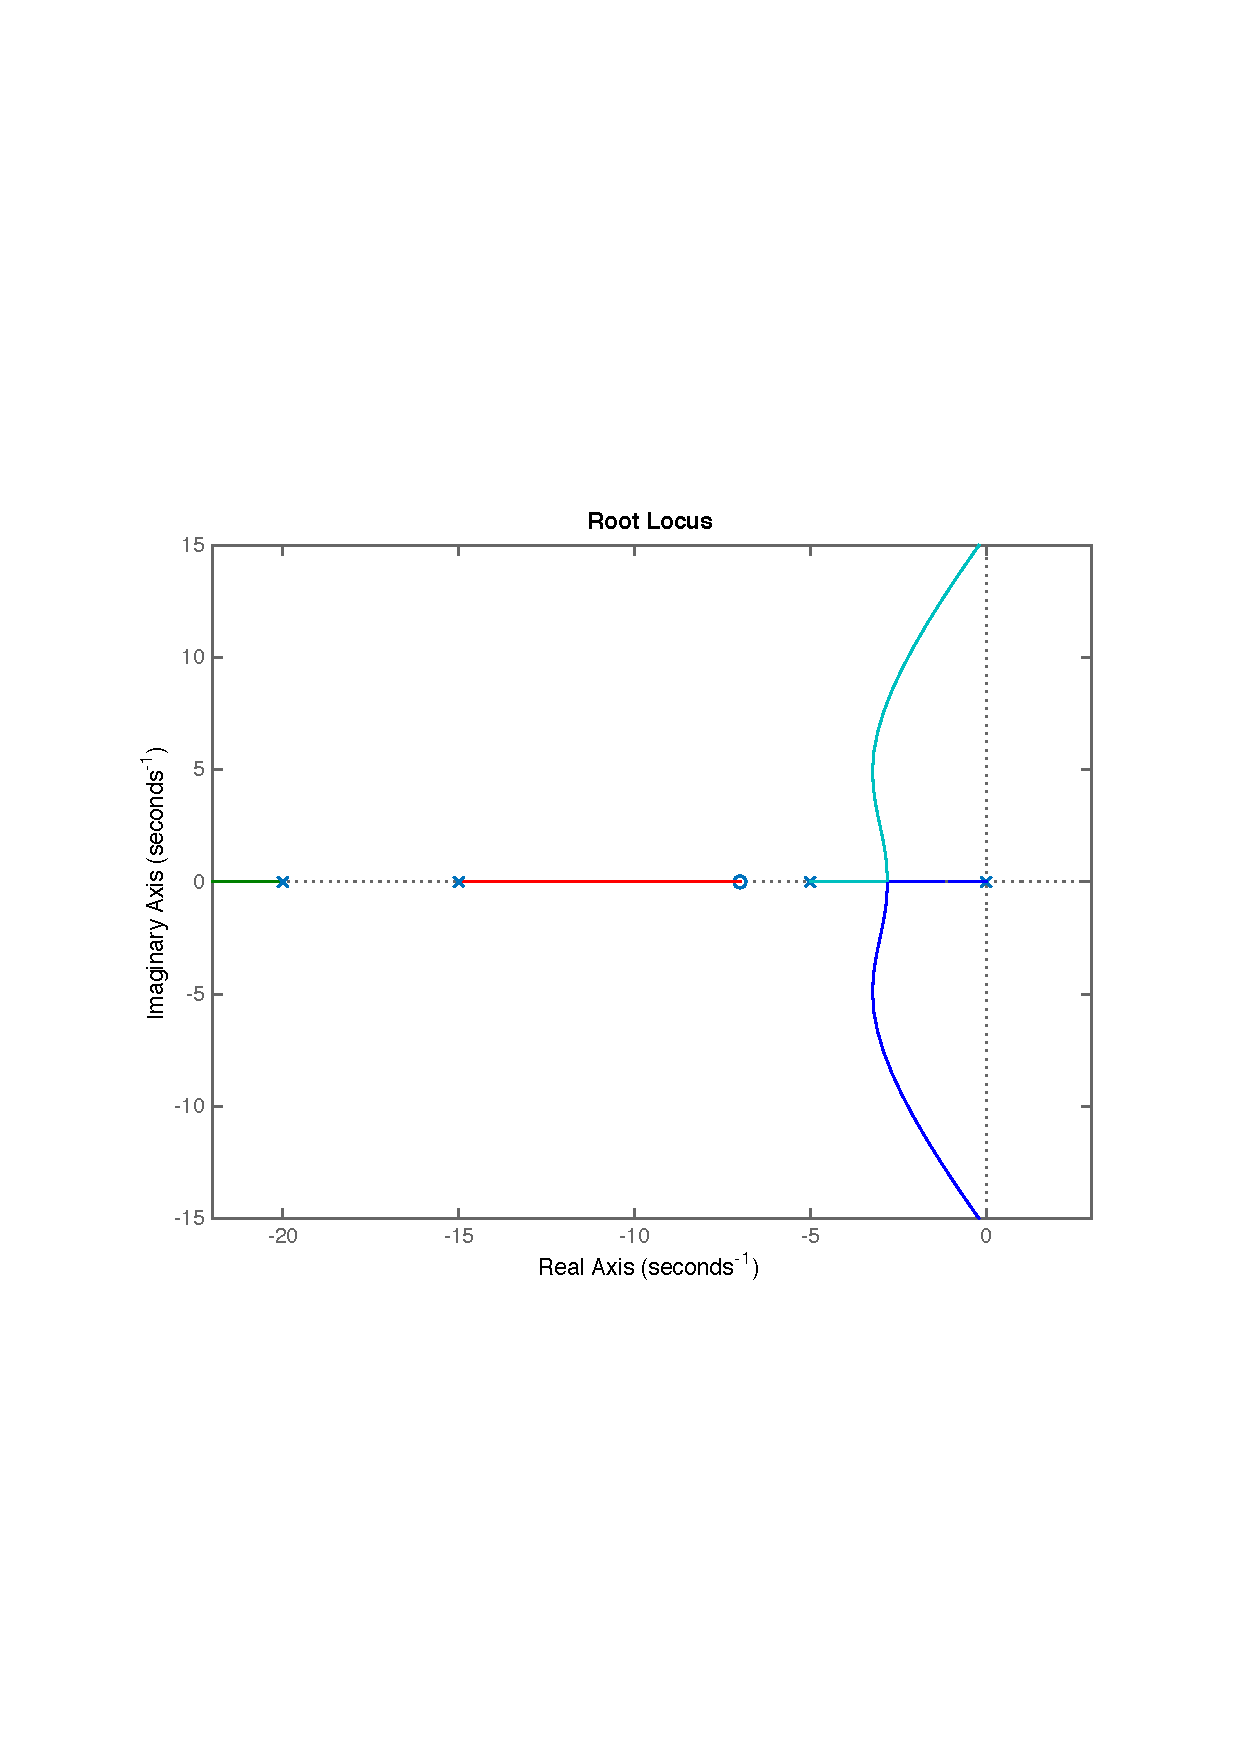
\includegraphics[width=0.7\linewidth]{matlab_ex1}
		\end{figure}
	\end{exampleblock}
\end{frame}

\begin{frame}
	\begin{exampleblock}{}
		Next we translate the design criteria into requirements for $\zeta$ and $\omega_n$:
		\begin{itemize}
			\item $\zeta = 0.7$;
			\item $\omega_n = 1.8$.
		\end{itemize}
		\vspace{1em}
		We can visualize these requirement using the \textbf{"sgrid(requirement1, requirement2,...)"}-command.\\
		\vspace{1em}
		MATLAB commands:\\
		Zeta = 0.7\\
		Wn = 1.8\\
		sgrid(Zeta, Wn)\\
	\end{exampleblock}
\end{frame}

\begin{frame}
	\begin{exampleblock}{}
		Which results in the following plot:
		\vspace{-0.5em}
		\begin{figure}
			\centering
			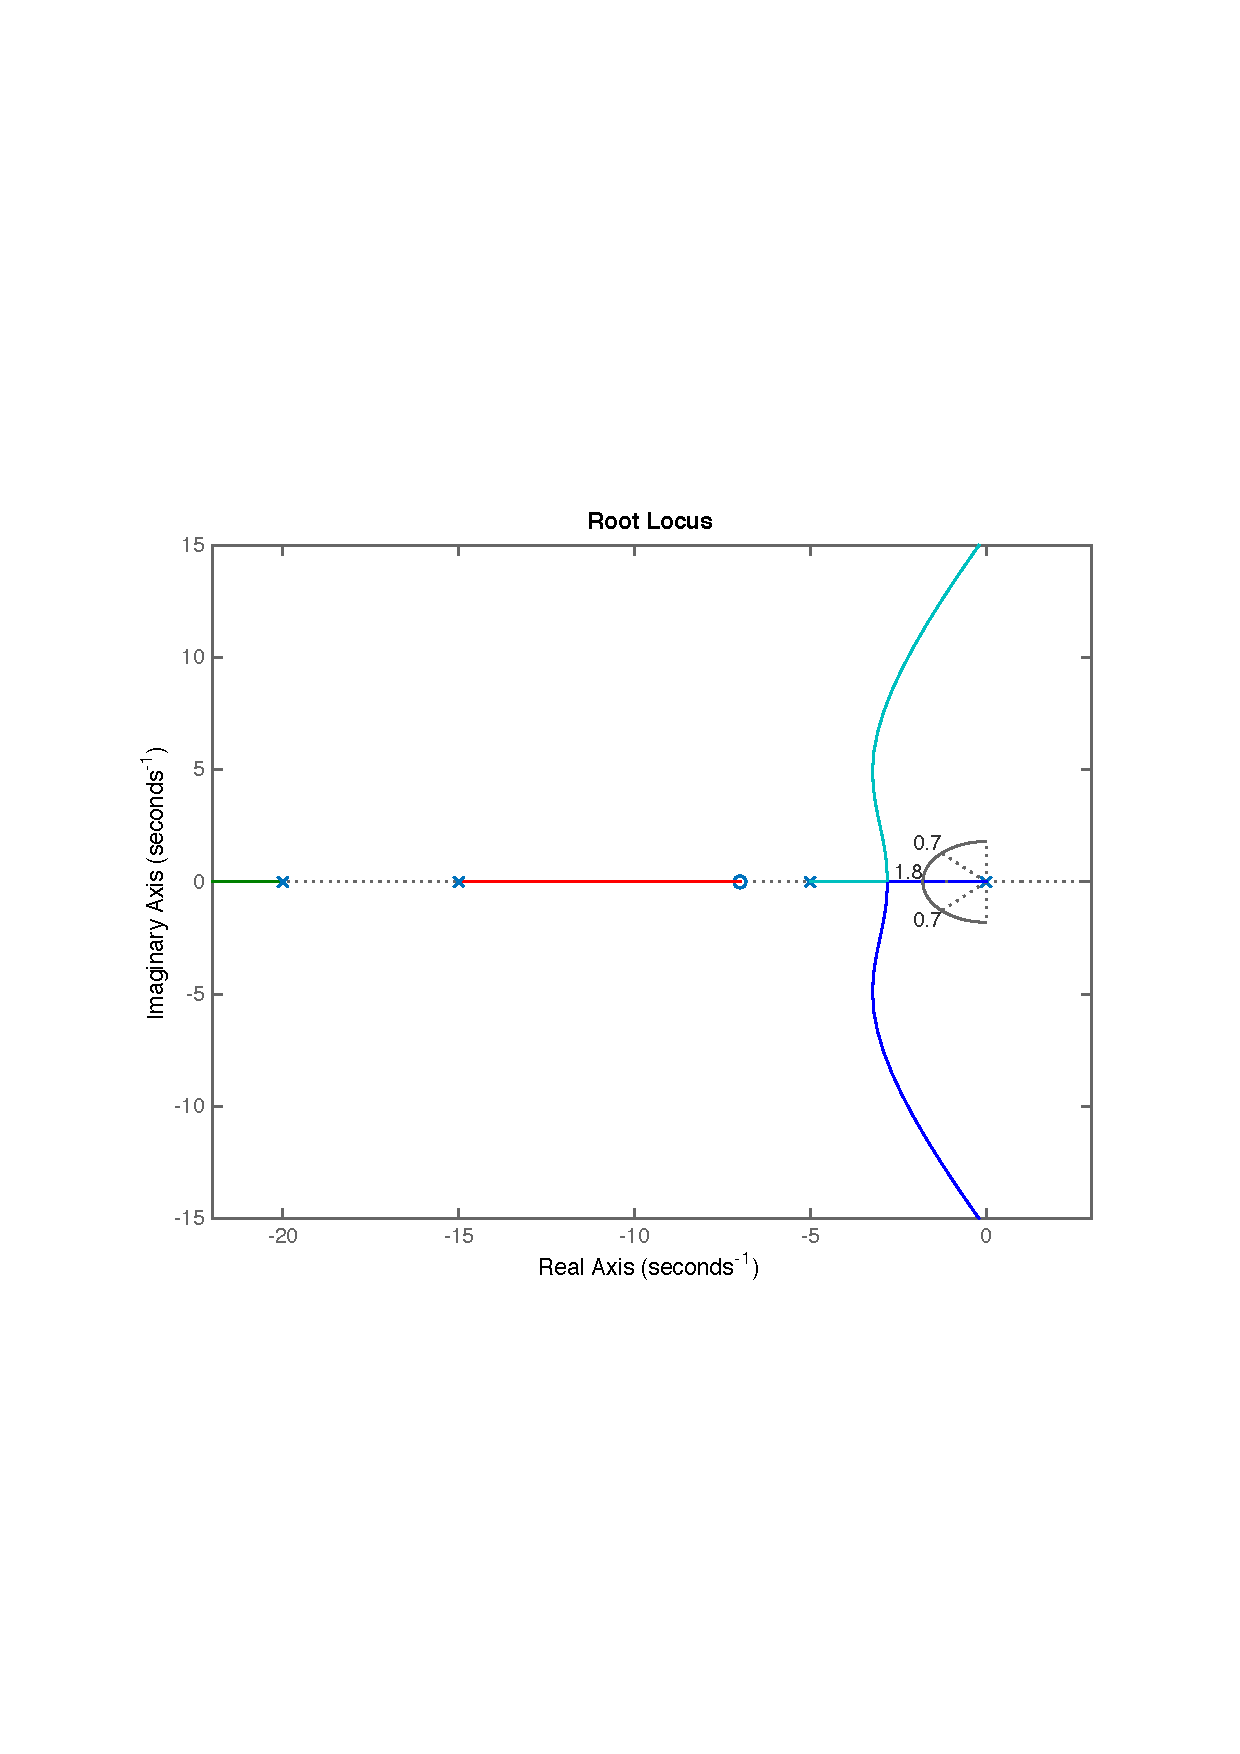
\includegraphics[width=0.7\linewidth]{matlab_ex2}
		\end{figure}
	\end{exampleblock}
\end{frame}

\begin{frame}
	\begin{exampleblock}{}
		Going back to our problem, to make the overshoot less than $5\%$, the poles have to be in between the two white dotted lines, and to make the rise time shorter than 1 second, the poles have to be outside of the white dotted semicircle.\\
		\vspace{1em}
		From the plot above we see that there is part of the root locus inside the desired region. So in this case, we need only a proportional controller to move the poles to the desired region. You can select a point on the root locus plot that meets the requirement by using the \textbf{"rlocfind(sys)"}-command.\\
		\vspace{1em}
		MATLAB command:\\
		[k,poles] = rlocfind(H)
	\end{exampleblock}
\end{frame}

\begin{frame}
	\begin{exampleblock}{}
		In the next figure, the \textcolor{red}{$+$}-sings indicate the selected points. MATLAB will return the gain and the poles of the system you have created by selecting these points.
		\vspace{-0.5em}
		\begin{figure}
			\centering
			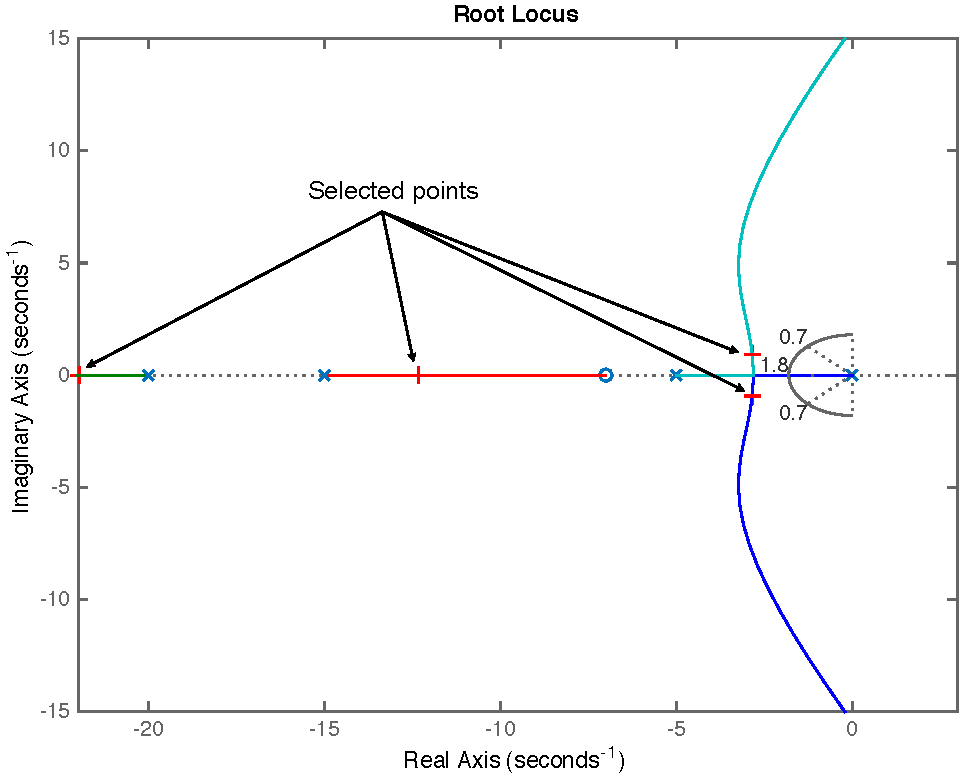
\includegraphics[width=0.6\linewidth]{matlab_ex3}
		\end{figure}
	\end{exampleblock}
\end{frame}

\subsection{SISOTOOL}

\begin{frame}
\frametitle{MATLAB Commands}
	Another way to visualize the root locus, is by using the interactive MATLAB GUI called sisotool. The SISO design tool is an interactive graphical user interface that facilitates the design of compensator for single-input, single-output (SISO) feedback loops.\\
	\vspace{1em}
	First you need to define your system in MATLAB and then you use the sisotool function on your system: \textbf{"sisotool(sys)"}. An interactive user face will pop up in which you can select you plant, the plots you would like to see and many other options.	
\end{frame}

\begin{frame}
\frametitle{MATLAB Commands}
	\begin{example}
		We can also design the same controller as done above but instead of using separate commands, we will now make use of the sisotool. 
		Same transfer function: $H(s) = \frac{s+7}{s(s+5)(s+15)(s+20)}$\\
		and the same design criteria: 
		\begin{itemize}
			\item overshoot must be less than $5\%$;
			\item rise time = $1s$
		\end{itemize}
		MATLAB commands:
		s = tf('s')\\
		plant = (s+7)/(s*(s+5)*(s+15)*(s+20)) \textcolor{gray}{we define the system H by its transfer function} \\
		sisotool(plant) \textcolor{gray}{we summon the sisotool, an interactive user face will pop up}\\ 
	\end{example}
\end{frame}

\begin{frame}
\frametitle{MATLAB Commands}
	\begin{exampleblock}{}
		In the \textbf{Control and Estimation Tools Manager} you can select the tab labeled \textbf{Graphical Tuning}. In this tab: 
		\begin{itemize}
			\item turn \textbf{Plot 2} off;
			\item make sure \textbf{Plot 1} is the root locus.
		\end{itemize}
		Now you can click the button labeled \textbf{Show Design Plot} and then a tunable plot will appear. In this root locus plot, you can drag the closed-loop poles along the locus to adjust the loop gain. 
	\end{exampleblock}
\end{frame}

\begin{frame}
\frametitle{MATLAB Commands}
	\begin{exampleblock}{}
		The following figures are an example of the result you get when you move the closed-loop poles.
	\begin{columns}
		\begin{column}{0.5\textwidth}
			\begin{figure}
				\centering
				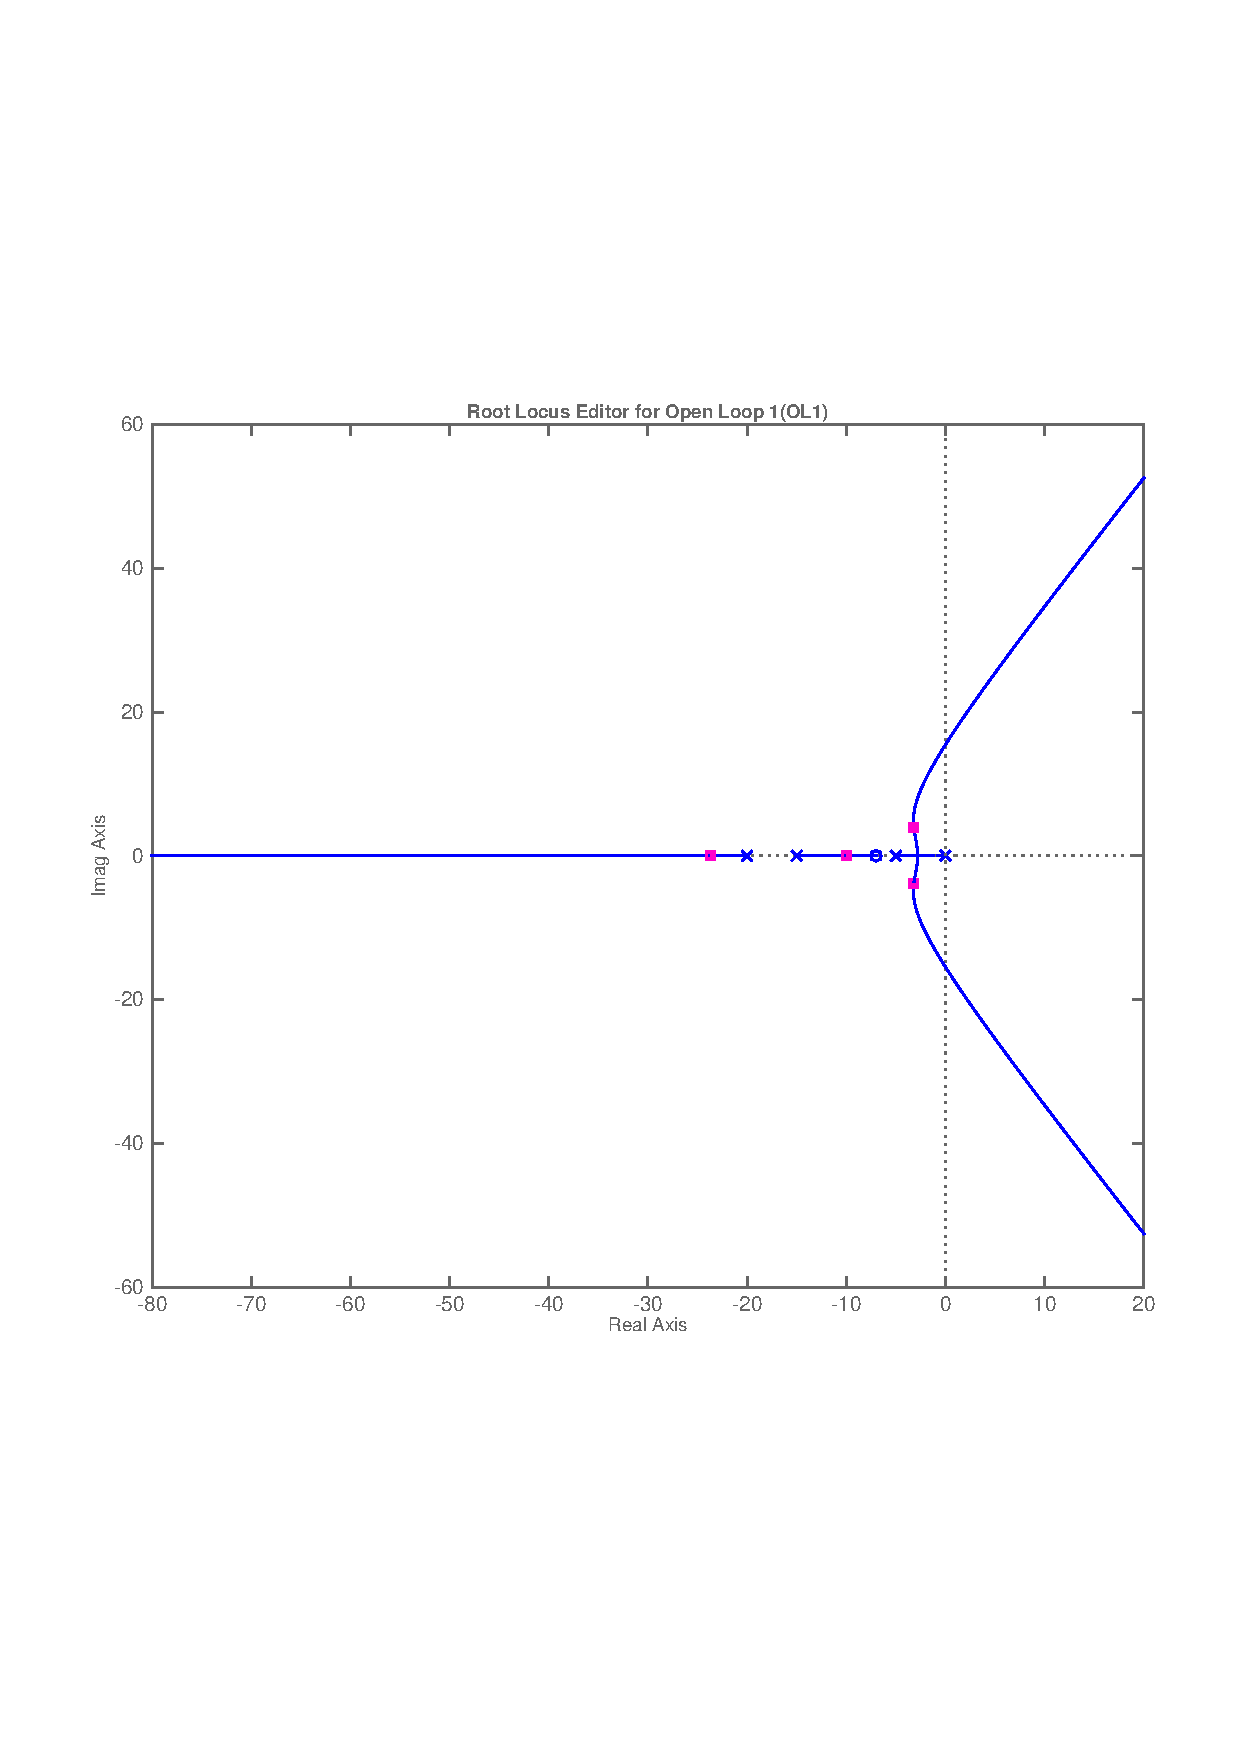
\includegraphics[width=0.9\linewidth]{matlab_ex4}
			\end{figure}
		\end{column}
		\begin{column}{0.5\textwidth}
			\begin{figure}
				\centering
				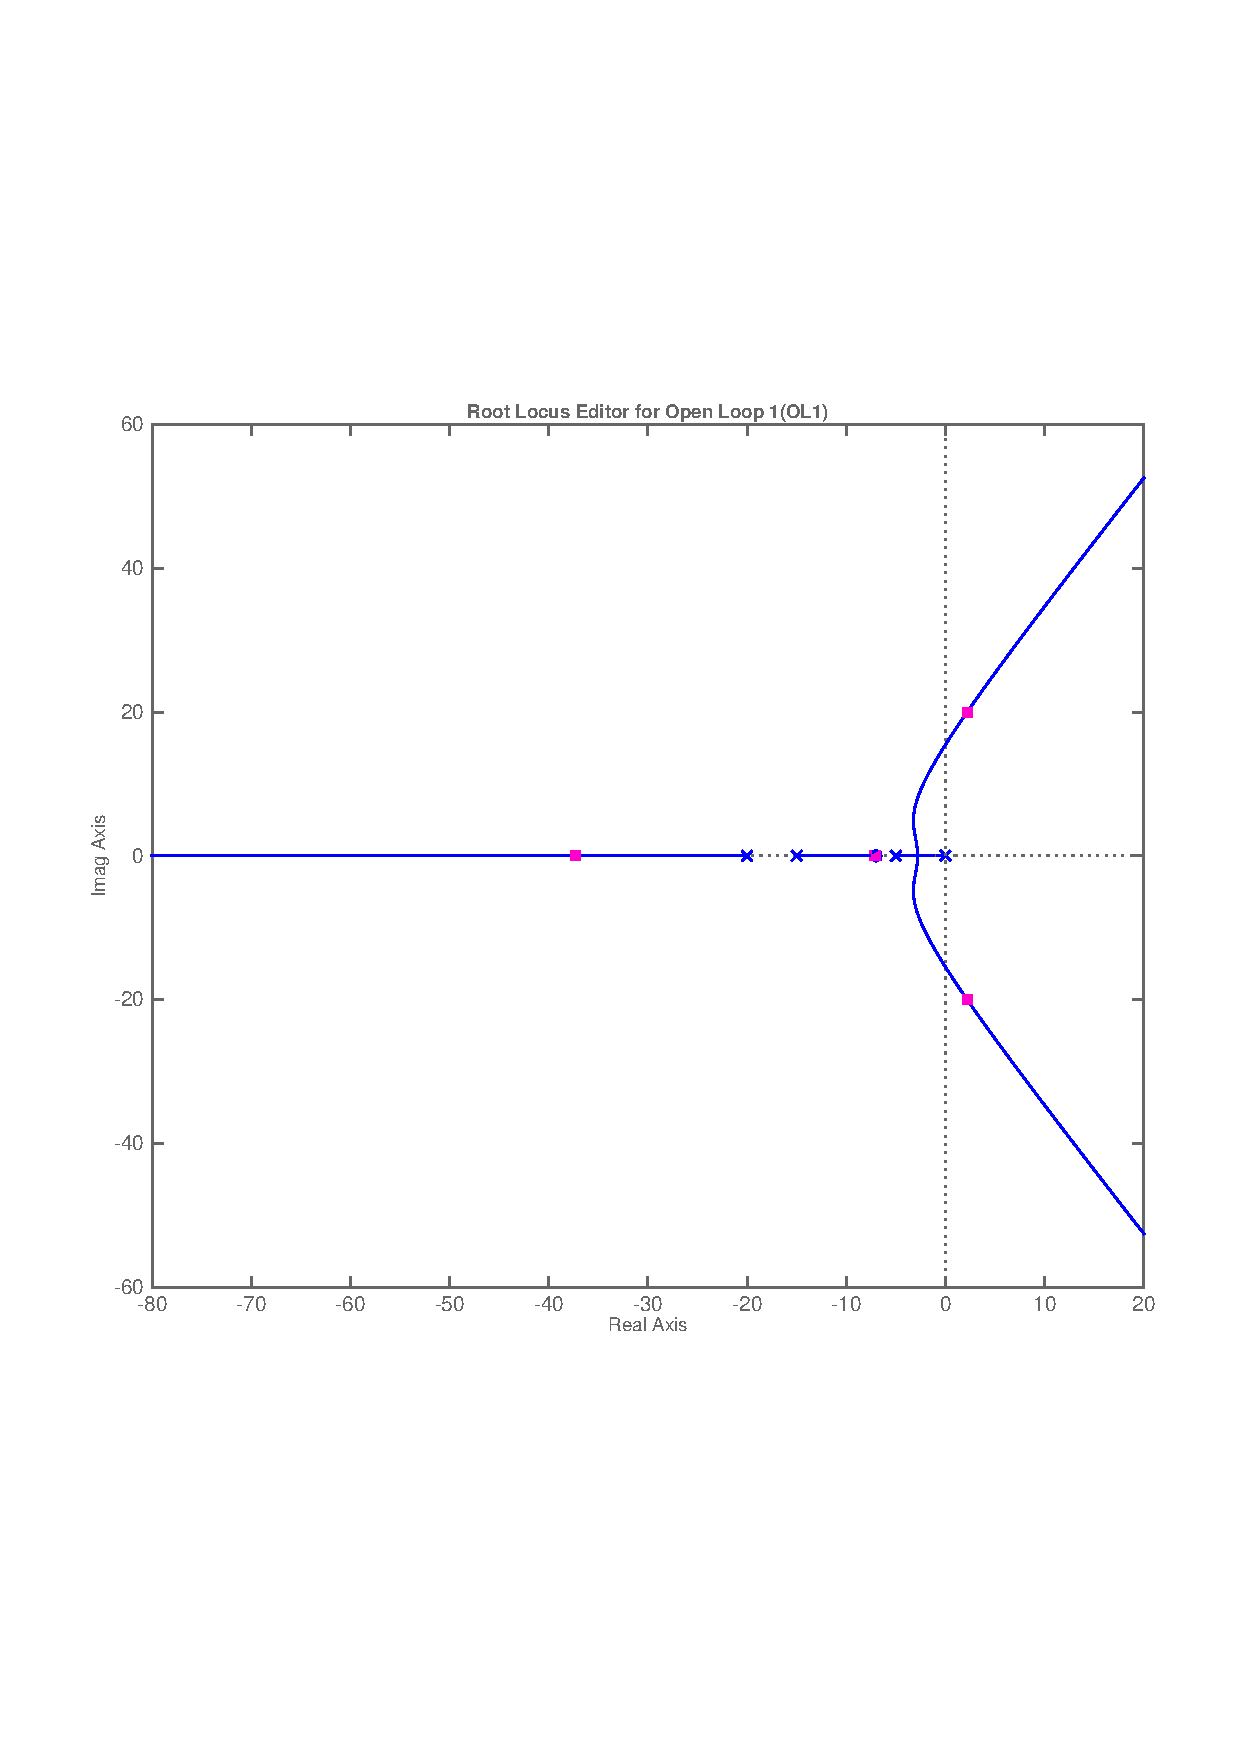
\includegraphics[width=0.9\linewidth]{matlab_ex5}
			\end{figure}
		\end{column}
	\end{columns}
	\end{exampleblock}
\end{frame}

\begin{frame}
\frametitle{MATLAB Commands}
	\begin{exampleblock}{}
		We can take the design criteria into account directly in the plot. This is done by right-clicking and selecting \textbf{Design Requirements, New}. Now you can specify the different design criteria: settling time, percent overshoot, damping ratio, natural frequency, region constant.\\
		\vspace{1em}
		In our example we have 2 design criteria which we have already translated into requirements for $\zeta$ and $\omega_n$: 
		\begin{itemize}
			\item $\zeta = 0.7$;
			\item $\omega_n = 1.8$.
		\end{itemize}
		\vspace{1em}
		On the plot, any area which is still white, is an acceptable region for the poles.
	\end{exampleblock}
\end{frame}

\begin{frame}
\frametitle{MATLAB Commands}
	\begin{exampleblock}{}
		If we complete the specification of the requirements and adjust the axis for a better view, we obtain the following figure:
		\begin{figure}
			\centering
			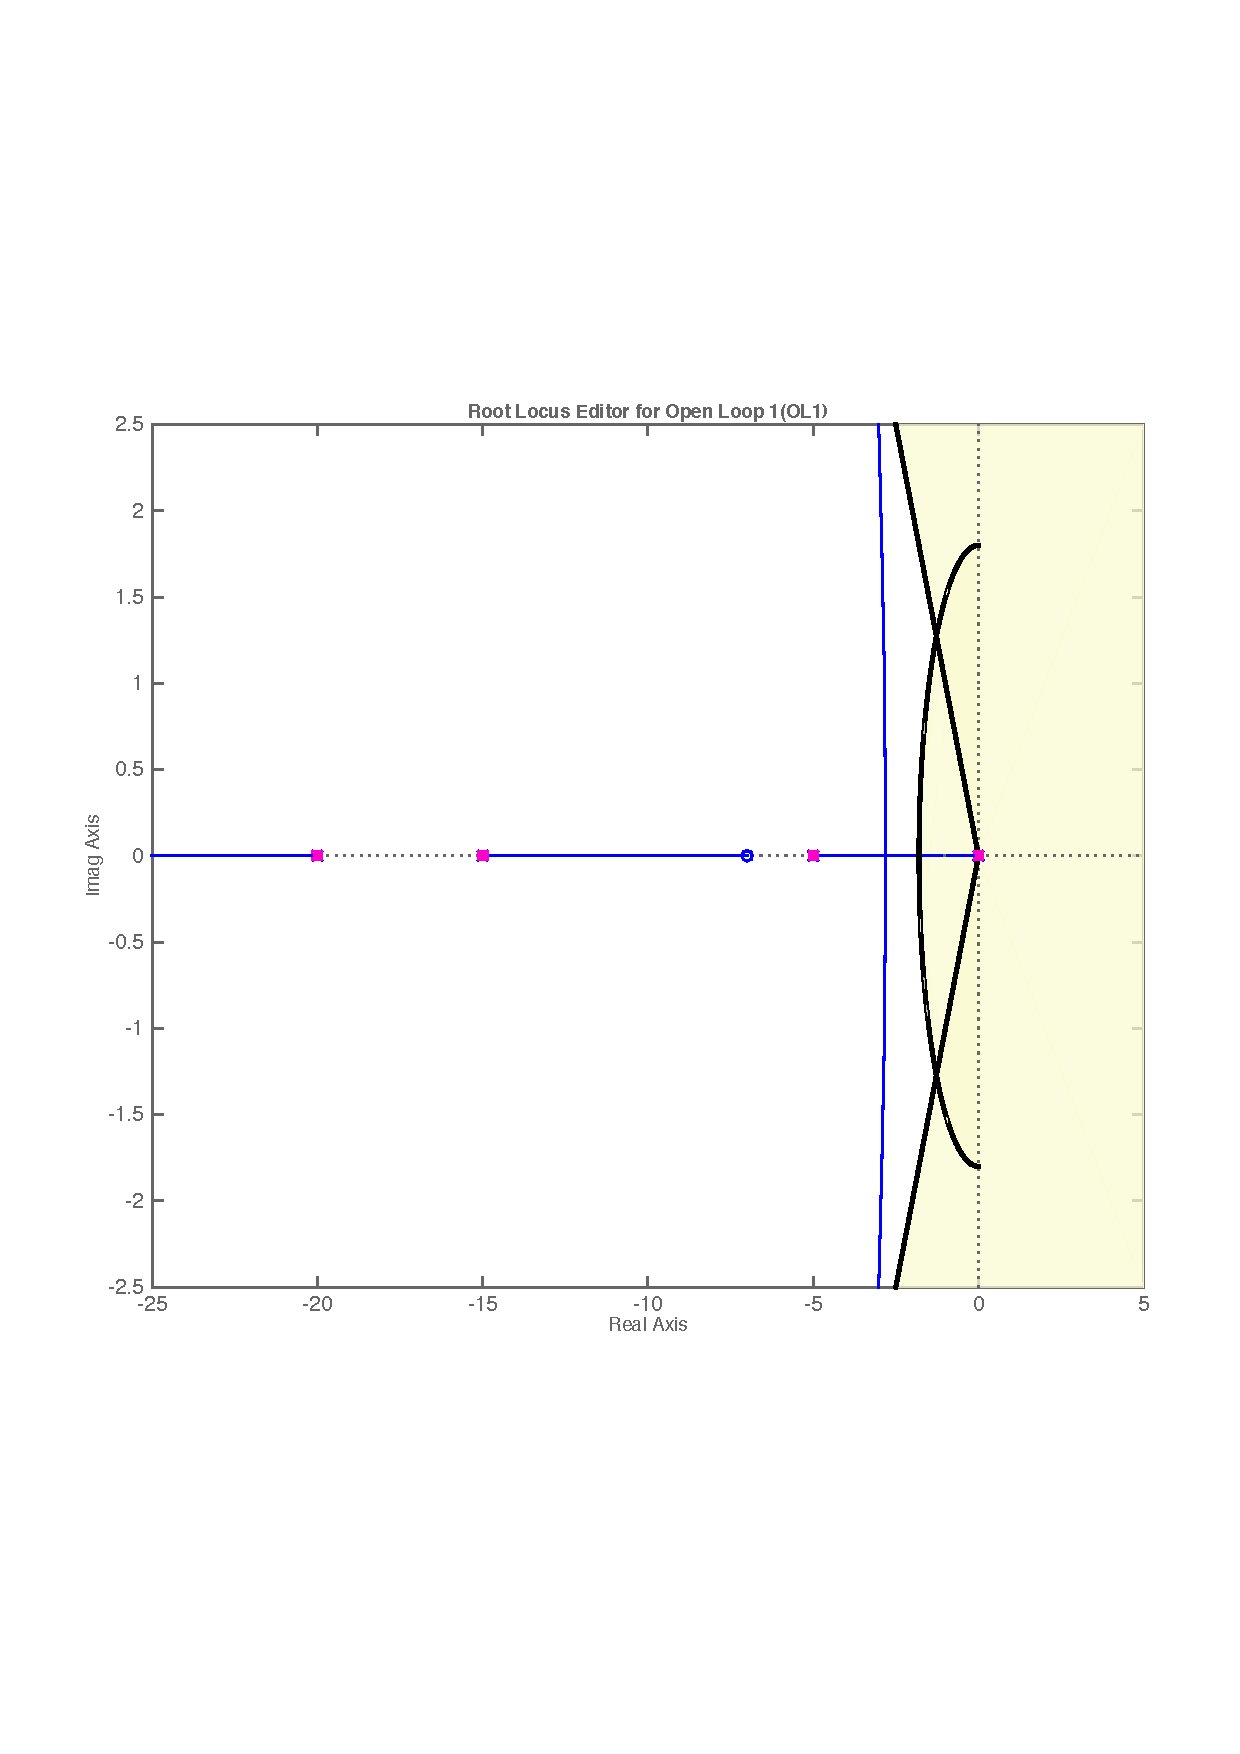
\includegraphics[width=0.5\linewidth]{matlab_ex6}
		\end{figure}
	\end{exampleblock}
\end{frame}
